
%%%%%%%%%%%%%%%%%%%%%%%%%%%%% Thesis.tex %%%%%%%%%%%%%%%%%%%%%%%%%%%%%%%
%                                                                      %
%  ---------- Master of Science Dissertation template ----------       %
%                                                                      %
%  Template for the Master Thesis according to the regulations         %
%  published by the Scientific Council at IST.                         %
%                                                                      %
%  For up-to-date regulations, please refer to                         %
%  http://cd.ist.utl.pt/files/publico/academicos/guia_dissertacao.pdf  %
%                                                                      %
%       Email: santiagorui14@gmail.com                                  %
%                                                                      %
%  Created:       Jan 20, 2015                                         %
%                                        %
%                                                                      %
%%%%%%%%%%%%%%%%%%%%%%%%%%%%%%%%%%%%%%%%%%%%%%%%%%%%%%%%%%%%%%%%%%%%%%%%
%  Revision history                                                    %
%  v1 - 2011/01/24 - original template                                 %
%  v2 - 2012/10/30 - new IST image and glossary support                %
%%%%%%%%%%%%%%%%%%%%%%%%%%%%%%%%%%%%%%%%%%%%%%%%%%%%%%%%%%%%%%%%%%%%%%%%
%                                                                      %
% To generate the PDF file, type "make" at the terminal prompt.        %
%                                                                      %
% The IST template LaTeX package was created by the author             %
% and it can be downloaded from:                                       %
% https://fenix.ist.utl.pt/homepage/ist31052/                          %
%                                                                      %
% The external packages can be downloaded from                         %
% the Comprehensive TeX Archive Network at http://www.ctan.org/        %
%                                                                      %
% List of LaTex symbols:                                               %
% http://www.ctan.org/tex-archive/info/symbols/comprehensive/          %
%                                                                      %
% Help with LaTex can be found at                                      %
% http://www.giss.nasa.gov/tools/latex/ltx-2.html                      %
% http://en.wikibooks.org/wiki/LaTeX                                   %
%%%%%%%%%%%%%%%%%%%%%%%%%%%%%%%%%%%%%%%%%%%%%%%%%%%%%%%%%%%%%%%%%%%%%%%%

%%%%%%%%%%%%%%%%%%%%%%%%%%%%%%%%%%%%%%%%%%%%%%%%%%%%%%%%%%%%%%%%%%%%%%%%
%     Preamble                                                         %
%%%%%%%%%%%%%%%%%%%%%%%%%%%%%%%%%%%%%%%%%%%%%%%%%%%%%%%%%%%%%%%%%%%%%%%%

% ----------------------------------------------------------------------
%  Set the document class
% ----------------------------------------------------------------------
\documentclass[10pt,a4paper,twoside]{report}
\usepackage{helvet}
\renewcommand{\familydefault}{\sfdefault}
\usepackage{setspace}
\onehalfspacing
\usepackage{indentfirst}
\usepackage{mathtools}
\usepackage{amsmath}
\usepackage{listings}


\usepackage{geometry}
 \geometry{
 a4paper,
 %total={210mm,297mm},
 left=25mm,
 right=25mm,
 top=25mm,
 bottom=25mm,
 }



% ----------------------------------------------------------------------
% Define external packages, language, margins, fonts and new commands
% ----------------------------------------------------------------------
%%%%%%%%%%%%%%%%%%%%%%%%%%%%%%%%%%%%%%%%%%%%%%%%%%%%%%%%%%%%%%%%%%%%%%%%
%                                                                      %
%     File: Thesis_Preamble.tex                                        %
%     Tex Master: Thesis.tex                                           %
%                                                                      %
%     Author: Gonçalo Santos                                           %
%     Last modified : 20 Oct 2018                                      %
%                                                                      %
%%%%%%%%%%%%%%%%%%%%%%%%%%%%%%%%%%%%%%%%%%%%%%%%%%%%%%%%%%%%%%%%%%%%%%%%

% ----------------------------------------------------------------------
% Define document language.
% ----------------------------------------------------------------------

% 'inputenc' package
%
% Accept different input encodings.
% http://www.ctan.org/tex-archive/macros/latex/base/
%
% > allows typing non-english text in LaTeX sources.
%
% ******************************* SELECT *******************************
%\usepackage[latin1]{inputenc} % <<<<< Windows
\usepackage[utf8]{inputenc}   % <<<<< Linux
% ******************************* SELECT *******************************


% 'babel' package
%
% Multilingual support for Plain TeX or LaTeX.
% http://www.ctan.org/tex-archive/macros/latex/required/babel/
%
% > sets the variable names according to the language selected
%
% ******************************* SELECT *******************************
%\usepackage[portuguese]{babel} % <<<<< Portuguese
\usepackage[english]{babel} % <<<<< English
% ******************************* SELECT *******************************


% List of LaTeX variable names: \abstractname, \appendixname, \bibname,
%   \chaptername, \contentsname, \listfigurename, \listtablename, ...
% http://www.tex.ac.uk/cgi-bin/texfaq2html?label=fixnam
%
% Changing the words babel uses (uncomment and redefine as necessary...)
%
\newcommand{\acknowledgments}{@undefined} % new LaTeX variable name
%
% > English
%
\addto\captionsenglish{\renewcommand{\acknowledgments}{Acknowledgments}}
%\addto\captionsenglish{\renewcommand{\listtablename}{List of Tables}}
%\addto\captionsenglish{\renewcommand{\listfigurename}{List of Figures}}
%\addto\captionsenglish{\renewcommand{\nomname}{Nomenclature}}
%\addto\captionsenglish{\renewcommand{\appendixname}{Appendix}}
%\addto\captionsenglish{\renewcommand{\bibname}{References}} % Bibliography

% > Portuguese
%
\addto\captionsportuguese{\renewcommand{\acknowledgments}{Agradecimentos}}
%\addto\captionsportuguese{\renewcommand{\listtablename}{Lista de Figuras}}
%\addto\captionsportuguese{\renewcommand{\listfigurename}{Lista de Tabelas}}
\addto\captionsportuguese{\renewcommand{\nomname}{Lista de S\'{i}mbolos}} % Nomenclatura
%\addto\captionsportuguese{\renewcommand{\appendixname}{Anexo}} % Apendice
%\addto\captionsportuguese{\renewcommand{\bibname}{Refer\^{e}ncias}} % Bibliografia


% ----------------------------------------------------------------------
% Define default and cover page fonts.
% ----------------------------------------------------------------------

% Use Arial font as default
%
\renewcommand{\rmdefault}{phv}
\renewcommand{\sfdefault}{phv}

% Define cover page fonts
%
%         encoding     family       series      shape
%  \usefont{T1}     {phv}=helvetica  {b}=bold    {n}=normal
%                   {ptm}=times      {m}=normal  {sl}=slanted
%                                                {it}=italic
% see more examples at
% http://julien.coron.free.fr/languages/latex/fonts/
%
\def\FontLn{% 16 pt normal
  \usefont{T1}{phv}{m}{n}\fontsize{16pt}{16pt}\selectfont}
\def\FontLb{% 16 pt bold
  \usefont{T1}{phv}{b}{n}\fontsize{16pt}{16pt}\selectfont}
\def\FontMn{% 14 pt normal
  \usefont{T1}{phv}{m}{n}\fontsize{14pt}{14pt}\selectfont}
\def\FontMb{% 14 pt bold
  \usefont{T1}{phv}{b}{n}\fontsize{14pt}{14pt}\selectfont}
\def\FontSn{% 12 pt normal
  \usefont{T1}{phv}{m}{n}\fontsize{12pt}{12pt}\selectfont}


% ----------------------------------------------------------------------
% Define page margins and line spacing.
% ----------------------------------------------------------------------

% 'geometry' package
%
% Flexible and complete interface to document dimensions.
% http://www.ctan.org/tex-archive/macros/latex/contrib/geometry/
%
% > set the page margins (2.5cm minimum in every side, as per IST rules)
%
\usepackage{geometry}	
\geometry{verbose,tmargin=2.5cm,bmargin=2.5cm,lmargin=2.5cm,rmargin=2.5cm}

% 'setspace' package
%
% Set space between lines.
% http://www.ctan.org/tex-archive/macros/latex/contrib/setspace/
%
% > allow setting line spacing (line spacing of 1.5, as per IST rules)
%
\usepackage{setspace}
\renewcommand{\baselinestretch}{1.5}


% ----------------------------------------------------------------------
% Include external packages.
% Note that not all of these packages may be available on all system
% installations. If necessary, include the .sty files locally in
% the <jobname>.tex file directory.
% ----------------------------------------------------------------------

% 'graphicx' package
%
% Enhanced support for graphics.
% http://www.ctan.org/tex-archive/macros/latex/required/graphics/
%
% > extends arguments of the \includegraphics command
%
\usepackage{graphicx}


% 'color' package
%
% Colour control for LaTeX documents.
% http://www.ctan.org/tex-archive/macros/latex/required/graphics/
%
% > defines color macros: \color{<color name>}
%
%\usepackage{color}


% 'amsmath' package
%
% Mathematical enhancements for LaTeX.
% http://www.ctan.org/tex-archive/macros/latex/required/amslatex/
%
% > American Mathematical Society plain Tex macros
%
\usepackage{amsmath}  % AMS mathematical facilities for LaTeX.
\usepackage{amsthm}   % Typesetting theorems (AMS style).
\usepackage{amsfonts} %


% 'wrapfig' package
%
% Produces figures which text can flow around.
% http://www.ctan.org/tex-archive/macros/latex/contrib/wrapfig/
%
% > wrap figures/tables in text (i.e., Di Vinci style)
%
% \usepackage{wrapfig}


% 'subfigure' package
%
% Deprecated: Figures divided into subfigures.
% http://www.ctan.org/tex-archive/obsolete/macros/latex/contrib/subfigure/
%
% > subcaptions for subfigures
%
\usepackage{subfigure}


% 'subfigmat' package
%
% Automates layout when using the subfigure package.
% http://www.ctan.org/tex-archive/macros/latex/contrib/subfigmat/
%
% > matrices of similar subfigures
%
\usepackage{subfigmat}


% 'url' package
%
% Verbatim with URL-sensitive line breaks.
% http://www.ctan.org/tex-archive/macros/latex/contrib/url/
%
% > URLs in BibTex
%
% \usepackage{url}


% 'varioref' package
%
% Intelligent page references.
% http://www.ctan.org/tex-archive/macros/latex/required/tools/
%
% > smart page, figure, table and equation referencing
%
%\usepackage{varioref}


% 'dcolumn' package
%
% Align on the decimal point of numbers in tabular columns.
% http://www.ctan.org/tex-archive/macros/latex/required/tools/
%
% > decimal-aligned tabular math columns
%
\usepackage{dcolumn}
\newcolumntype{d}{D{.}{.}{-1}} % column aligned by the point separator '.'
\newcolumntype{e}{D{E}{E}{-1}} % column aligned by the exponent 'E'


% '' package
%
% Reimplementation of and extensions to LaTeX verbatim.
% http://www.ctan.org/tex-archive/macros/latex/required/tools/
%
% > provides the verbatim environment (\begin{verbatim},\end{verbatim})
%   and a comment environment (\begin{comment},  \end{comment})
%
% \usepackage{verbatim}


% 'moreverb' package
%
% Extended verbatim.
% http://www.ctan.org/tex-archive/macros/latex/contrib/moreverb/
%
% > supports tab expansion and line numbering
%
% \usepackage{moreverb}



% 'nomencl' package
%
% Produce lists of symbols as in nomenclature.
% http://www.ctan.org/tex-archive/macros/latex/contrib/nomencl/
%
% The nomencl package makes use of the MakeIndex program
% in order to produce the nomenclature list.
%
% Nomenclature
% 1: On running the file through LATEX, the command \makenomenclature
%    in the preamble instructs it to create/open the nomenclature file
%    <jobname>.nlo corresponding to the LATEX file <jobname>.tex and
%    writes the information from the \nomenclature commands to this file.
% 2: The next step is to invoke MakeIndex in order to produce the
%    <jobname>.nls file. This can be achieved by making use of the
%    command: makeindex <jobname>.nlo -s nomencl.ist -o <jobname>.nls
% 3: The last step is to invoke LATEX on the <jobname>.tex file once
%    more. There, the \printnomenclature in the document will input the
%    <jobname>.nls file and process it according to the given options.
%
% http://www-h.eng.cam.ac.uk/help/tpl/textprocessing/nomencl.pdf
%
% Nomenclature (produces *.nlo *.nls files)
\usepackage{nomencl}
\makenomenclature
%
% Group variables according to their symbol type
%
\RequirePackage{ifthen}
\ifthenelse{\equal{\languagename}{english}}%
    { % English
    \renewcommand{\nomgroup}[1]{%
      \ifthenelse{\equal{#1}{R}}{%
        \item[\textbf{Roman symbols}]}{%
        \ifthenelse{\equal{#1}{G}}{%
          \item[\textbf{Greek symbols}]}{%
          \ifthenelse{\equal{#1}{S}}{%
            \item[\textbf{Subscripts}]}{%
            \ifthenelse{\equal{#1}{T}}{%
              \item[\textbf{Superscripts}]}{}}}}}%
    }{% Portuguese
    \renewcommand{\nomgroup}[1]{%
      \ifthenelse{\equal{#1}{R}}{%
        \item[\textbf{Simbolos romanos}]}{%
        \ifthenelse{\equal{#1}{G}}{%
          \item[\textbf{Simbolos gregos}]}{%
          \ifthenelse{\equal{#1}{S}}{%
            \item[\textbf{Subscritos}]}{%
            \ifthenelse{\equal{#1}{T}}{%
              \item[\textbf{Sobrescritos}]}{}}}}}%
    }%


% 'glossary' package
%
% Create a glossary.
% http://www.ctan.org/tex-archive/macros/latex/contrib/glossary/
%
% Glossary (produces *.glo *.ist files)
\usepackage[number=none]{glossary}
% (remove blank line between groups)
\setglossary{gloskip={}}
% (redefine glossary style file)
%\renewcommand{\istfilename}{myGlossaryStyle.ist}
\makeglossary


% 'rotating' package
%
% Rotation tools, including rotated full-page floats.
% http://www.ctan.org/tex-archive/macros/latex/contrib/rotating/
%
% > show wide figures and tables in landscape format:
%   use \begin{sidewaystable} and \begin{sidewaysfigure}
%   instead of 'table' and 'figure', respectively.
%
\usepackage{rotating}


% 'hyperref' package
%
% Extensive support for hypertext in LaTeX.
% http://www.ctan.org/tex-archive/macros/latex/contrib/hyperref/
%
% > Extends the functionality of all the LATEX cross-referencing
%   commands (including the table of contents, bibliographies etc) to
%   produce \special commands which a driver can turn into hypertext
%   links; Also provides new commands to allow the user to write adhoc
%   hypertext links, including those to external documents and URLs.
%
\usepackage[pdftex]{hyperref} % enhance documents that are to be
                              % output as HTML and PDF
\hypersetup{colorlinks,       % color text of links and anchors,
                              % eliminates borders around links
%            linkcolor=red,    % color for normal internal links
            linkcolor=black,  % color for normal internal links
            anchorcolor=black,% color for anchor text
%            citecolor=green,  % color for bibliographical citations
            citecolor=black,  % color for bibliographical citations
%            filecolor=magenta,% color for URLs which open local files
            filecolor=black,  % color for URLs which open local files
%            menucolor=red,    % color for Acrobat menu items
            menucolor=black,  % color for Acrobat menu items
%            pagecolor=red,    % color for links to other pages
            pagecolor=black,  % color for links to other pages
%            urlcolor=cyan,    % color for linked URLs
            urlcolor=black,   % color for linked URLs
	          bookmarks=true,         % create PDF bookmarks
	          bookmarksopen=false,    % don't expand bookmarks
	          bookmarksnumbered=true, % number bookmarks
	          pdftitle={Thesis},
            pdfauthor={Andre C. Marta},
            pdfsubject={Thesis Title},
            pdfkeywords={Thesis Keywords},
            pdfstartview=FitV,
            pdfdisplaydoctitle=true}


% 'hypcap' package
%
% Adjusting the anchors of captions.
% http://www.ctan.org/tex-archive/macros/latex/contrib/oberdiek/
%
% > fixes the problem with hyperref, that links to floats points
%   below the caption and not at the beginning of the float.
%
\usepackage[figure,table]{hypcap}


% 'natbib' package
%
% Flexible bibliography support.
% http://www.ctan.org/tex-archive/macros/latex/contrib/natbib/
%
% > produce author-year style citations
%
% \citet  and \citep  for textual and parenthetical citations, respectively
% \citet* and \citep* that print the full author list, and not just the abbreviated one
% \citealt is the same as \citet but without parentheses. Similarly, \citealp is \citep without parentheses
% \citeauthor
% \citeyear
% \citeyearpar
%
\usepackage{natbib}


% ----------------------------------------------------------------------
% Define new commands to assure consistent treatment throughout document
% ----------------------------------------------------------------------

\newcommand{\ud}{\mathrm{d}}                % total derivative
\newcommand{\degree}{\ensuremath{^\circ\,}} % degrees

% Abbreviations

\newcommand{\mcol}{\multicolumn}            % table format

\newcommand{\eqnref}[1]{(\ref{#1})}
\newcommand{\class}[1]{\texttt{#1}}
\newcommand{\package}[1]{\texttt{#1}}
\newcommand{\file}[1]{\texttt{#1}}
\newcommand{\BibTeX}{\textsc{Bib}\TeX}

% Typefaces ( example: {\bf Bold text here} )
%
% > pre-defined
%   \bf % bold face
%   \it % italic
%   \tt % typewriter
%
% > newly defined
\newcommand{\tr}[1]{{\ensuremath{\textrm{#1}}}}   % text roman
\newcommand{\tb}[1]{{\ensuremath{\textbf{#1}}}}   % text bold face
\newcommand{\ti}[1]{{\ensuremath{\textit{#1}}}}   % text italic
\newcommand{\mc}[1]{{\ensuremath{\mathcal{#1}}}}  % math calygraphy
\newcommand{\mco}[1]{{\ensuremath{\mathcalold{#1}}}}% math old calygraphy
\newcommand{\mr}[1]{{\ensuremath{\mathrm{#1}}}}   % math roman
\newcommand{\mb}[1]{{\ensuremath{\mathbf{#1}}}}   % math bold face
\newcommand{\bs}[1]{\ensuremath{\boldsymbol{#1}}} % math symbol
\def\bm#1{\mathchoice                             % math bold
  {\mbox{\boldmath$\displaystyle#1$}}%
  {\mbox{\boldmath$#1$}}%
  {\mbox{\boldmath$\scriptstyle#1$}}%
  {\mbox{\boldmath$\scriptscriptstyle#1$}}}
\newcommand{\boldcal}[1]{{\ensuremath{\boldsymbol{\mathcal{#1}}}}}% math bold calygraphy

\usepackage{fancyvrb}
 % file "Thesis_Preamble.tex"
%%%%%%%%%%%%%%%%%%%%%%%%%%%%%%%%%%%%%%%%%%%%%%%%%%%%%%%%%%%%%%%%%%%%%%%%
%     Begin Document                                                   %
%%%%%%%%%%%%%%%%%%%%%%%%%%%%%%%%%%%%%%%%%%%%%%%%%%%%%%%%%%%%%%%%%%%%%%%%
\begin{document}

% Set plain page style (no headers, footer with centered page number)
\pagestyle{plain}

% Set roman numbering (i,ii,...) before the start of chapters
\pagenumbering{roman}

% ----------------------------------------------------------------------
%  Cover page
% ----------------------------------------------------------------------
%%%%%%%%%%%%%%%%%%%%%%%%%%%%%%%%%%%%%%%%%%%%%%%%%%%%%%%%%%%%%%%%%%%%%%%%
%                                                                      %
%     File: Thesis_FrontCover.tex                                      %
%     Tex Master: Thesis.tex                                           %
%                                                                      %
%     Author: Gonçalo Santos                                           %
%     Last modified : 20 Oct 2018                                      %
%                                                                      %
%%%%%%%%%%%%%%%%%%%%%%%%%%%%%%%%%%%%%%%%%%%%%%%%%%%%%%%%%%%%%%%%%%%%%%%%

\thispagestyle {empty}

% IST Logo
% parameters: bb=llx lly urx ury (bounding box), width=h_length, height=v_length, angle=angle, scale=factor, clip=true/false, draft=true/false.
\vspace*{-12mm}
\hspace*{-12mm}

\includegraphics[height=20mm]{IST_A_CMYK_POS-crop.pdf}

\begin{center}
%
% Figure (Image or plot)
\vspace{0.5cm}
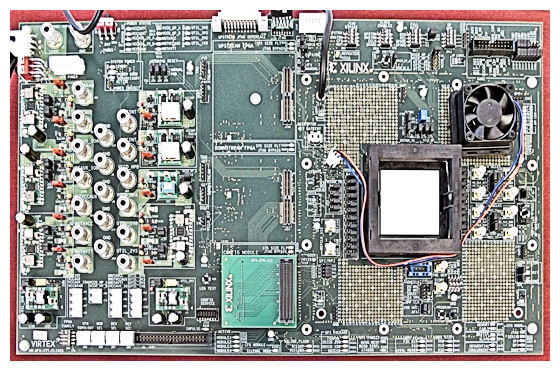
\includegraphics[height=60mm]{Figures/fpga.jpg}

% Title, author and degree
\vspace{0.8cm}
{\FontLb C Compiler for the VERSAT Reconfigurable Processor} \\
\vspace{3.6cm}
{\FontMb Gonçalo da Conceição Reis dos Santos} \\
\vspace{1.9cm}
{\FontLn Thesis to obtain the Master of Science Degree in} \\
\vspace{0.3cm}
{\FontLb Electrical and Computer Engineering} \\
%\vspace{1.9cm}
\vspace{1.0cm}
{\FontSn %
\begin{tabular}{ll}
Supervisor: & Prof. José João Henriques Teixeira de Sousa
\end{tabular} } \\
\vspace{1.0cm}
{\FontMb Examination Committee} \\
\vspace{0.3cm}
{\FontSn %
\begin{tabular}{ll}
Chairperson: & Prof. Francisco André Corrêa Alegria\\
Supervisor: & Prof. José João Henriques Teixeira de Sousa \\
Member of the Committee: & Prof. Paulo Ferreira Godinho Flores \\
\end{tabular} } \\
\vspace{1.5cm}
{\FontMb November 2019} \\
%
\end{center}

\cleardoublepage
 % file "Thesis_FrontCover.tex"

% ----------------------------------------------------------------------
% Dedication page (optional)
% ----------------------------------------------------------------------
%%%%%%%%%%%%%%%%%%%%%%%%%%%%%%%%%%%%%%%%%%%%%%%%%%%%%%%%%%%%%%%%%%%%%%%%%
%                                                                      %
%     File: Thesis_Dedication.tex                                      %
%     Tex Master: Thesis.tex                                           %
%                                                                      %
%     Author: Andre C. Marta                                           %
%     Last modified :  2 Jul 2015                                      %
%                                                                      %
%%%%%%%%%%%%%%%%%%%%%%%%%%%%%%%%%%%%%%%%%%%%%%%%%%%%%%%%%%%%%%%%%%%%%%%%

\null\vskip5cm%
\begin{flushright}
     Dedicated to someone special...
\end{flushright}
\vfill\newpage

 % file "Thesis_Dedication.tex"

% ----------------------------------------------------------------------
%  Acknowledgments (optional)
% ----------------------------------------------------------------------
%%%%%%%%%%%%%%%%%%%%%%%%%%%%%%%%%%%%%%%%%%%%%%%%%%%%%%%%%%%%%%%%%%%%%%%%%
%                                                                      %
%     File: Thesis_Acknowledgments.tex                                 %
%     Tex Master: Thesis.tex                                           %
%                                                                      %
%     Author: Andre C. Marta                                           %
%     Last modified :  2 Jul 2015                                      %
%                                                                      %
%%%%%%%%%%%%%%%%%%%%%%%%%%%%%%%%%%%%%%%%%%%%%%%%%%%%%%%%%%%%%%%%%%%%%%%%

\section*{\acknowledgments}

% Add entry in the table of contents as section
\addcontentsline{toc}{section}{\acknowledgments}

I want to thank my supervisor, Professor José Teixeira de Sousa, for the 
opportunity to develop this work and for his guidance and support during that process. 
His help was fundamental to overcome the multiple obstacles that I faced during this work.

I also want to acknowledge Professor Horácio Neto for providing a simple Convolutional 
Neural Network application, used as a basis for the application developed for the 
RV32-Versat architecture.

A special acknowledgement goes to my friends, for their continuous support, and Válter,  
that is developing a multi-layer architecture for RV32-Versat. When everything seemed to 
be doomed he always had a miraculous solution.

Finally, I want to express my sincere gratitude to my family for giving me all the 
support and encouragement that I needed throughout my years of study and through the 
process of researching and writing this thesis. They are also part of this work.\\

\textbf{Thank you.}

 % file "Thesis_Acknowledgements.tex"

% ----------------------------------------------------------------------
%  Abstract (both in English and Portuguese)
% ----------------------------------------------------------------------
%%%%%%%%%%%%%%%%%%%%%%%%%%%%%%%%%%%%%%%%%%%%%%%%%%%%%%%%%%%%%%%%%%%%%%%%%
%                                                                      %
%     File: Thesis_Resumo.tex                                          %
%     Tex Master: Thesis.tex                                           %
%                                                                      %
%     Author: Carlos A. Rodrigues                                           %
%     Last modified : 21 Jan 2011                                      %
%                                                                      %
%%%%%%%%%%%%%%%%%%%%%%%%%%%%%%%%%%%%%%%%%%%%%%%%%%%%%%%%%%%%%%%%%%%%%%%%

\section*{Resumo}

% Add entry in the table of contents as section
\addcontentsline{toc}{section}{Resumo}

Inserir o resumo em Portugu\^{e}s aqui com o máximo de 250 palavras e acompanhado de 4 a 6 palavras-chave...

\vfill

\textbf{\Large Palavras-chave:} OpenRISC, Sistema em um chip,...

\cleardoublepage

 % file "Thesis_Resumo.tex"
%%%%%%%%%%%%%%%%%%%%%%%%%%%%%%%%%%%%%%%%%%%%%%%%%%%%%%%%%%%%%%%%%%%%%%%%%
%                                                                      %
%     File: Thesis_Abstract.tex                                        %
%     Tex Master: Thesis.tex                                           %
%                                                                      %
%     Author: Andre C. Marta                                           %
%     Last modified :  2 Jul 2015                                      %
%                                                                      %
%%%%%%%%%%%%%%%%%%%%%%%%%%%%%%%%%%%%%%%%%%%%%%%%%%%%%%%%%%%%%%%%%%%%%%%%

\section*{Abstract}

% Add entry in the table of contents as section
\addcontentsline{toc}{section}{Abstract}

Versat is a Coarse-Grain Reconfigurable Array architecture (CGRA), which
implements self and partial reconfiguration by using a simple controller
unit. This report studies the current state of the art in HDL and CGRA
simulation, providing a basis to the development of a simulation environment for
Versat. The main objective of this environment is to provide a faster way to
develop and debug software without the use of prototyping hardware. Therefore,
the two types of HDL simulators, event-driven and cycle-accurate, their
advantages and disadvantages are studied, along with a performance comparison
between them. A study of high-level implementations for CGRA simulation is
also presented.

\vfill

\textbf{\Large Keywords:} Versat, coarse-grain reconfigurable arrays, HDL
simulation, CGRA simulation, high-level simulation

 % file "Thesis_Abstract.tex"

% ----------------------------------------------------------------------
%  Table of contents, list of tables, list of figures and nomenclature
% ----------------------------------------------------------------------

% Table of contents
%
\tableofcontents
\cleardoublepage 

% List of tables
%
% Generate list
\listoftables
% Add entry in the table of contents as section
\addcontentsline{toc}{section}{\listtablename}
\cleardoublepage 

% List of figures
%
% Generate list
\listoffigures
% Add entry in the table of contents as section
\addcontentsline{toc}{section}{\listfigurename}
\cleardoublepage 

%% Nomenclature
%%
%% entries of nomenclature list
%%%%%%%%%%%%%%%%%%%%%%%%%%%%%%%%%%%%%%%%%%%%%%%%%%%%%%%%%%%%%%%%%%%%%%%%%
%                                                                      %
%     File: Thesis_Nomenclature.tex                                    %
%     Tex Master: Thesis.tex                                           %
%                                                                      %
%     Author: Gonçalo Santos                                           %
%     Last modified : 20 Oct 2018                                      %
%                                                                      %
%%%%%%%%%%%%%%%%%%%%%%%%%%%%%%%%%%%%%%%%%%%%%%%%%%%%%%%%%%%%%%%%%%%%%%%%
%
% The definitions can be placed anywhere in the document body
% and their order is sorted by <symbol> automatically when
% calling makeindex in the makefile
%
% The \glossary command has the following syntax:
%
% \glossary{entry}
%
% The \nomenclature command has the following syntax:
%
% \nomenclature[<prefix>]{<symbol>}{<description>}
%
% where <prefix> is used for fine tuning the sort order,
% <symbol> is the symbol to be described, and <description> is
% the actual description.

% ----------------------------------------------------------------------
% Roman symbols [r]
\nomenclature[ru]{$\bf u$}{Velocity vector.}
\nomenclature[ru]{$u,v,w$}{Velocity Cartesian components.}
\nomenclature[rp]{$p$}{Pressure.}
\nomenclature[rC]{$C_D$}{Coefficient of drag.}
\nomenclature[rC]{$C_L$}{Coefficient of lift.}
\nomenclature[rC]{$C_M$}{Coefficient of moment.}

% ----------------------------------------------------------------------
% Greek symbols [g]
\nomenclature[g]{$\rho$}{Density.}
\nomenclature[g]{$\alpha$}{Angle of attack.}
\nomenclature[g]{$\beta$}{Angle of side-slip.}
\nomenclature[g]{$\mu$}{Molecular viscosity coefficient.}
\nomenclature[g]{$\kappa$}{Thermal conductivity coefficient.}

% ----------------------------------------------------------------------
% Subscripts [s]
\nomenclature[s]{$x,y,z$}{Cartesian components.}
\nomenclature[s]{$i,j,k$}{Computational indexes.}
\nomenclature[s]{$\infty$}{Free-stream condition.}
\nomenclature[s]{ref}{Reference condition.}
\nomenclature[s]{$n$}{Normal component.}

% ----------------------------------------------------------------------
% Supercripts [t]
\nomenclature[t]{T}{Transpose.}
\nomenclature[t]{*}{Adjoint.}

 % file "Thesis_Nomenclature.tex"
%%
%% Insert glossary/nomenclature section produced by MakeIndex
%\printnomenclature
%% Add entry in the table of contents as section
%\addcontentsline{toc}{section}{\nomname}
%\cleardoublepage

% entries of glossary list
%%%%%%%%%%%%%%%%%%%%%%%%%%%%%%%%%%%%%%%%%%%%%%%%%%%%%%%%%%%%%%%%%%%%%%%%%
%                                                                      %
%     File: Thesis_Glossary.tex                                        %
%     Tex Master: Thesis.tex                                           %
%                                                                      %
%     Author: Carlos A. Rodrigues                                           %
%     Last modified : 30 Oct 2012                                      %
%                                                                      %
%%%%%%%%%%%%%%%%%%%%%%%%%%%%%%%%%%%%%%%%%%%%%%%%%%%%%%%%%%%%%%%%%%%%%%%%
%
% The definitions can be placed anywhere in the document body
% and their order is sorted by <symbol> automatically when
% calling makeindex in the makefile
%
% The \glossary command has the following syntax:
%
% \glossary{entry}
%
% The \nomenclature command has the following syntax:
%
% \nomenclature[<prefix>]{<symbol>}{<description>}
%
% where <prefix> is used for fine tuning the sort order,
% <symbol> is the symbol to be described, and <description> is
% the actual description.

% ----------------------------------------------------------------------

\glossary{name={\textbf{MDO}},description={Multi-Disciplinar Optimization is an engineering technique that uses optimization methods to solve design problems incorporating two or more disciplines.}}

\glossary{name={\textbf{CFD}},description={Computational Fluid Dynamics is a branch of fluid mechanics that uses numerical methods and algorithms to solve problems that involve fluid flows.}}

\glossary{name={\textbf{CSM}},description={Computational Structural Mechanics is a branch of structure mechanics that uses numerical methods and algorithms to perform the analysis of structures and its components.}}

 % file "Thesis_Glossary.tex"

% Insert glossary section produced by MakeIndex
%\printglossary
% Add entry in the table of contents as section
%\addcontentsline{toc}{section}{\glossaryname}
%\cleardoublepage


% Set arabic numbering (1,2,...) after preface
%
\setcounter{page}{1}
\pagenumbering{arabic}

% ----------------------------------------------------------------------
%  Chapters
% ----------------------------------------------------------------------

%%%%%%%%%%%%%%%%%%%%%%%%%%%%%%%%%%%%%%%%%%%%%%%%%%%%%%%%%%%%%%%%%%%%%%%%
%                                                                      %
%     File: Thesis_Introduction.tex                                    %
%     Tex Master: Thesis.tex                                           %
%                                                                      %
%     Author: Andre C. Marta                                           %
%     Last modified :  2 Jul 2015                                      %
%                                                                      %
%%%%%%%%%%%%%%%%%%%%%%%%%%%%%%%%%%%%%%%%%%%%%%%%%%%%%%%%%%%%%%%%%%%%%%%%

\chapter{Introduction}
\label{chapter:introduction}




In this report, the problem of accelerating the execution of Deep Neural
Networks (DNNs) using Coarse GRained Reconfigurable Arrays (CGRAs) is studied,
with special emphasis on compiling a DNN description into code that runs on
CPU/CGRA system. The Deep Versat Architecture~\cite{valter:deepversat} CGRA will be used as an
implementation tool in this work.


%%%%%%%%%%%%%%%%%%%%%%%%%%%%%%%%%%%%%%%%%%%%%%%%%%%%%%%%%%%%%%%%%%%%%%%%
\section{Problem}
\label{section:problem}

Neural Networks have been an object of study since the 1940's, but until the
beginning of this decade their applications were limited and did not play a
major role in computer vision conferences. With its meteoric rise in research,
several solutions to accelerate this algorithm have appeared, from Field Programmable Gate Arrays (FPGA) to
Application Specific Integrated Circuits (ASIC) implementations.

Convolutional Neural Networks (CNNs) are a particular kind of DNN where the output
values of the neurons in one layer are convolved with a kernel to produce the
input values of the neurons of the next layer. This algorithm is compute bound,
that is, its performance depends on how fast it can do certain calculations, and
depend less on the memory access time. Namely the convolutional layers take
approximately 90$\%$ of the computation time.

The acceleration of these workloads is a matter of importance for today's
applications such as image processing for object recognition or simply to
enhance certain images. Other uses like instant translation and virtual
assistants are applications of neural networks and their acceleration is of
vital importance to bring them into Internet of Things.

A suitable circuit to accelerate DNNs in hardware is the CGRA. A CGRA is a
collection of Functional Units and memories with programmable interconnections
in order to form computational datapaths. A CGRA can be implemented in both
FPGAs and ASICs. CGRAs can be reconfigured much faster than FPGAs, as they have
much less configuration bits. If reconfiguration is done at runtime, CGRAs add
temporal scalability to the spacial scalability that characterize
FPGAs. Moreover, partial reconfiguration is much easier to do in CGRAs compared
to FPGAs which further speeds up reconfiguration time. Another advantage of
CGRAs is the fact that they can be programmed entirely in software, contrasting
with the large development time of customized Intellectual Property (IP) blocks.
The Coarse Grain Reconfigurable Arrays (CGRA) is a midway acceleration solution
between FPGAs, which are flexible but large, power hungry and difficult to
reprogram, and ASICs, which are fast but generally not programmable.

However, mapping a specific DNN to a CGRA requires knowledge of its
architecture, latencies and register configurations, which may become a lengthy
process, especially if the user wants to explore the design space for several
DNN configurations. An automatic compiler that can map a standard DNN
description into CPU/CGRA code would dramatically decrease time to market of its
users. Currently there are equivalent tools for CPUs and GPUs and
even for FPGAS.


%%%%%%%%%%%%%%%%%%%%%%%%%%%%%%%%%%%%%%%%%%%%%%%%%%%%%%%%%%%%%%%%%%%%%%%%
\section{Solution}
\label{section:solution}

The proposed solution is a compiler that takes a configuration file from a
neural network framework like Caffe or Darknet. This new tool inputs the
parameters of Deep Versat, such as the number of layers and functional units,
and produces the C code needed for the Versat runs. This code is run on the
RISC-V picorv32~\cite{picorv} CPU controller that has Deep Versat as a peripheral.

%%%%%%%%%%%%%%%%%%%%%%%%%%%%%%%%%%%%%%%%%%%%%%%%%%%%%%%%%%%%%%%%%%%%%%%%
%\section{Thesis Outline}
%\label{section:outline}

%Briefly explain the contents of the different chapters...

%%%%%%%%%%%%%%%%%%%%%%%%%%%%%%%%%%%%%%%%%%%%%%%%%
%\section{Author's Work}
%\label{section:authorwork}

%TO ADD----

%%%%%%%%%%%%%%%%%%%%%%%%%%%%%%%%%%%%%%%%%%%%%%%%%%
\section{Report Outline}
\label{reportoutline}

This report is composed of 4 more chapters. In the second chapter, the
state-of-the-art of neural networks and the difficulties accelerating them is
described. In the third chapter, the Deep Versat architecture and how to program
it is explained. In the fourth chapter, CNN compiler techniques are
explored. Finally, the last chapter contains the proposed solution and the plan
for its execution.


 % file "Thesis_Introduction.tex"

%%%%%%%%%%%%%%%%%%%%%%%%%%%%%%%%%%%%%%%%%%%%%%%%%%%%%%%%%%%%%%%%%%%%%%%%
%                                                                      %
%     File: Thesis_Introduction.tex                                    %
%     Tex Master: Thesis.tex                                           %
%                                                                      %
%     Author: Rui Santiago                         			   %
%     Last modified : 4 Junho 2015                      		   %
%                                                                      %
%%%%%%%%%%%%%%%%%%%%%%%%%%%%%%%%%%%%%%%%%%%%%%%%%%%%%%%%%%%%%%%%%%%%%%%%


\chapter{Trabalho anterior}
\label{chapter:Trabalho anterior}

%O sistema num chip em inglês System On Chip \acrlong{soc} é um chip integrado que tem integrado todas as funcionalidades de computador ou de um sistema electrónico, num único chip. Um \acrshort{soc} é constituído tipicamente por vários elementos interligados entre si por um barramento. Os elementos podem ser separados por grupos conformes os seus principais funcionalidades, os principais grupos são os seguintes: processamento, memoria, fontes de \textcolor[rgb]{1,0,0}{timing}, periféricos, interfaces externas, interfaces analógicas e gestores de energia. Na figura \ref{figures:ARM} pode se um exemplo de um diagrama de blocos de um \acrshort{soc}, onde se pode o barramento ligação dos elementos.
As { \it Coarse Grain Reconfigurable Arrays} (CGRAs) ganharam atenção nas duas últimas décadas \cite{Mei05,Lee00,Weinhardt03,Quax04,deSousa12}. As CGRAs são estruturas de hardware programável que podem ser construídas com conjuntos de processadores RISC ou apenas com componentes simples como ALUs, multiplicadores, shifters\cite{Tripp07,deSousa12}. As arquitecturas CGRA permitem normalmente reduzir o consumo de energia.
%\setlength{\parskip}{1 cm}
                  
O desenvolvimento de geradores de endereços capazes de suportar ciclos encadeados numa única configuração permitiu reduzir o tempo de reconfiguração das CGRAs\cite{deSutter10}. A ideia foi inspirada no uso de contadores em cascata para o gerador de endereços\cite{Carta06}. 
                         
Existem dois tipos de configuração: a configuração estática e a configuração dinâmica (reconfiguração). Na configuração estática o sistema é configurado uma única vez para correr um programa completo, o que é menos flexível\cite{Hartenstein01}. Na configuração dinâmica pode-se reconfigurar o sistema multiplas vezes durante um programa. No entanto, é necessário contabilizar o tempo de reconfiguração de modo que o desempenho seja satisfatório. 
                             
Existem dois tipos de sistemas reconfiguráveis: homogéneos e heterogéneos. No sistema homogéneo, todas as unidades de processamento são idênticas\cite{Ebeling96}, e permitem realizar um leque alargado de funções. No caso dos sistemas heterogéneos, cada unidade realiza uma tarefa específica\cite{Heysters03}. Apesar das redes homogéneas potêncialmente serem mais eficientes, as redes heterogéneas compensam com um rácio de uso de silício melhor e com uma melhor utilização energética\cite{Park12}. 
                          
Um compilador para este tipo de arquitecturas não pode usar apenas técnicas convencionais, mas também precisa de usar técnicas de colocação de componentes e encaminhamento de sinais ({\it Place and Route}), usadas também em FPGAs\cite{Betz99}.  
                          
%\vfill\newpage

\cleardoublepage
%\begin{figure}[!htb]
 % \centering
 % 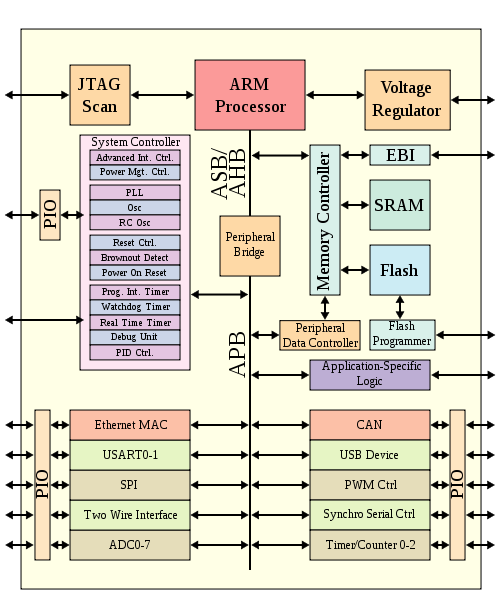
\includegraphics[width=0.5\textwidth]{Figures/ARM_SOC.png}
 % \caption[Diagrama de blocos de um soc ARM ]{Diagrama de blocos de um soc ARM }
 % \label{figures:ARM}
  %http://en.wikipedia.org/wiki/System_on_a_chip
%\end{figure}

%Os \acrshort{soc} têm uma vasta possibilidade de utilização desde um simples relógio até no mais avançado tecnologicamente como no desenvolvimentos de módulos para satélites, passando pela industria automóvel e com o aparecimento do arduino cada vez mais os \acrshort{soc} são utilizados em projetos de pequena escala desenvolvidos em casa, porque veio permitir a pessoas de com pouco ou nenhum conhecimento na área programar e efectuar debug no seu projecto com o \acrshort{soc}. A sua utilização traz vantagens com preço baixo, baixo consumo de energia e dimensões pequenas, como tudo o que existe também tem desvantagens sendo neste caso o baixo poder de calculo comparado com um computador. %http://www.extremetech.com/computing/126235-soc-vs-cpu-the-battle-for-the-future-of-computing

%Com uma área tão vasta de aplicações não é de estranhar que existam várias empresas \textcolor[rgb]{1,0,0}{a muito tempo} e varias startup no mercado a desenvolver \acrshort{soc} para fins totalmente distintos, cada empresa optimizando o seu para que foi desenvolvido.



% --------------------------------------------------------------------- 
%\section{Objectivos}
%\label{section:context}

%Uma startup no desenvolvimento de um projecto/produto necessita de um \acrshort{soc} para poder comercializar o seu produto. Na pesquisa do \acrshort{soc} ideal para o seu projecto encontram diferentes possibilidades, mas nenhuma preenchia todos os critérios pretendidos para o projecto. Como não foi encontrada uma solução ideal dos vários \acrshort{soc} disponíveis no mercado, a solução possível serias desenvolver o seu próprio \acrshort{soc} desenvolvido a medidas para o projecto.

% ----------------------------------------------------------------------
%\section{Motiva\c{c}\~ao}
%\label{section:motiva}

%\textcolor[rgb]{0,0,1}{desenvolver um sistema necessário para uma startup, o sistema vai ser desenvolvido a medida com o pretendido com a startup.}

%\section{Objectivos}
%\label{section:objectivo}

%A startup no desenvolvimento de um projeto/produto necessita de um \acrshort{soc}, como se pode ver na figura \ref{grafos:problema} que tem de ter a capacidade de processamento necessária para efetuar a descodificação e codificação de dados que irá receber e enviar. O \acrshort{soc} desenvolvido tem de permitir que sejas ligado mais dois modelos assíncronos permitindo a recolha de dados no local para posterior envio dos dados pelo modelo de comunicação. O produto é para ser usado em locais de difíceis acessos este terá de ter um baixo consumo, permitindo que a bateria funcione o maior tempo possível. Para alem do mencionado anteriormente também necessita de duas interfaces de comunicação \acrlong{uart} e \acrlong{gpio}. 

%\begin{figure}[!htb]
 % \centering
 % 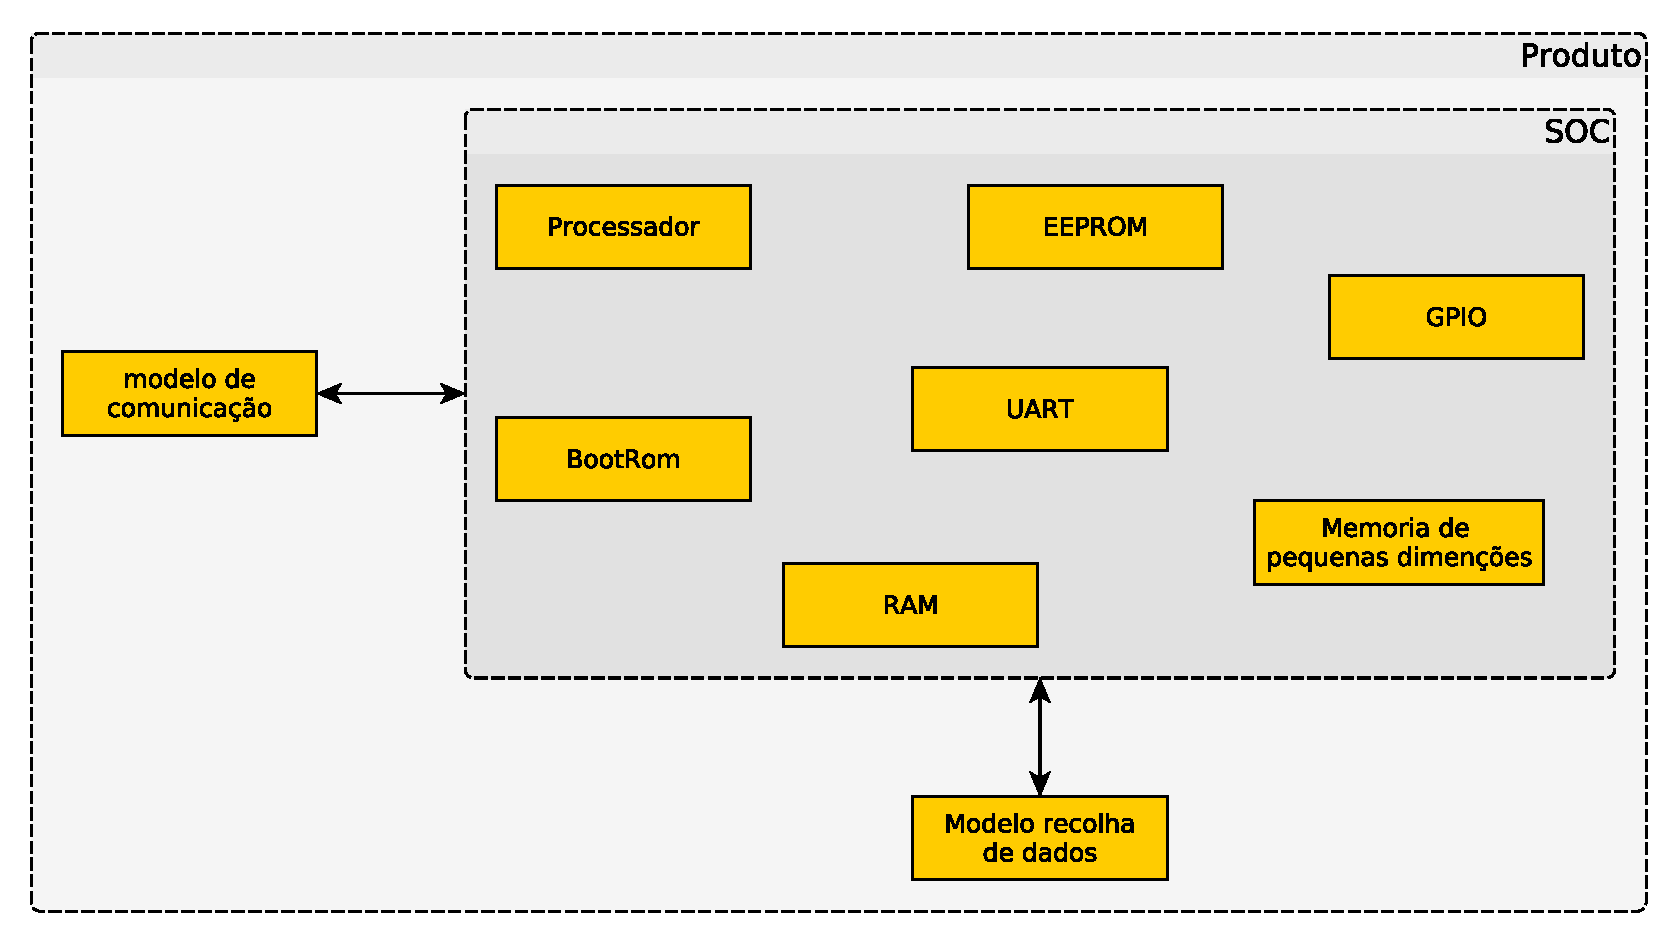
\includegraphics[width=0.5\textwidth]{grafos/problema.pdf}
 % \caption[SOC pretendido pela Startup]{SOC pretendido pela Startup}
 % \label{grafos:problema}
  %http://en.wikipedia.org/wiki/System_on_a_chip
%\end{figure}


%\section{Desafios}
%\label{section:desafio}


%Os principais desafios desta dissertação consiste no desenvolvimento de um sistema sintetizável que preencha todas as necessidades mencionadas pela startup.

%Desenvolver uma interface assíncrona necessária para a comunicação entre o \acrshort{soc} e os modelos de comunicação e de recolha de dados a ser desenvolvido pela startup.

%A criação de uma bootrom que carregua para a memoria principal o programa que se encontra na EEPROM. Ainda testa o mau funcionamento da EEPROM ou da memoria principal notificando o utilizador. 
 % file "Thesis_Estado_da_arte.tex"

%%%%%%%%%%%%%%%%%%%%%%%%%%%%%%%%%%%%%%%%%%%%%%%%%%%%%%%%%%%%%%%%%%%%%%%%
%                                                                      %
%     File: Thesis_Introduction.tex                                    %
%     Tex Master: Thesis.tex                                           %
%                                                                      %
%     Author: Rui Santiago                         			   %
%     Last modified : 2 Junho 2015                         		   %
%                                                                      %
%%%%%%%%%%%%%%%%%%%%%%%%%%%%%%%%%%%%%%%%%%%%%%%%%%%%%%%%%%%%%%%%%%%%%%%%
\chapter{Arquitectura do Versat}
\label{chapter:Arquitectura do Versat}
\setlength{\parskip}{0 cm}
%O sistema num chip em inglês System On Chip \acrlong{soc} é um chip integrado que tem integrado todas as funcionalidades de computador ou de um sistema electrónico, num único chip. Um \acrshort{soc} é constituído tipicamente por vários elementos interligados entre si por um barramento. Os elementos podem ser separados por grupos conformes os seus principais funcionalidades, os principais grupos são os seguintes: processamento, memoria, fontes de \textcolor[rgb]{1,0,0}{timing}, periféricos, interfaces externas, interfaces analógicas e gestores de energia. Na figura \ref{figures:ARM} pode se um exemplo de um diagrama de blocos de um \acrshort{soc}, onde se pode o barramento ligação dos elementos.
O Versat usa uma arquitectura {\it Coarse Grain Reconfigurable Arrays} (CGRAs). As arquitecturas CGRA surgiram com o objectivo de reduzir a complexidade, o tempo de configuração e o tempo de compilação em relação às arquitecturas FPGA. 

Todas as CGRAs possuem elementos de processamento (ALUs, multiplicadores, etc), onde são realizadas as operações. Também possuem uma rede de interconexão, que é usada para unir os vários elementos de processamento e memórias que armazenam configurações da arquitectura. As CGRAs variam em relação ao tipo de unidades de processamento utlizadas e à respectiva rede de interconexão. 


Dado que os sistemas homogéneos causam um desperdício de recursos, o Versat usa unidades de processamento heterogéneas. 
Para a realização da interconexão, as estruturas com nós todos conectados uns com os outros têm sido evitadas, visto que têm escalabilidade pobre em termos de área, um atraso entre os nós maior e um consumo maior. 
No entanto, no caso do Versat é usada esta topologia, pois é privilegiada a flexibilidade de configuração face à escalabilidade. Cada sistema Versat utiliza um número reduzido de nós, prevendo-se que a escalabilidade passe pela utilização de multiplos sistemas Versat em vez de um sistema Versat de grandes dimensões.
O facto de ser utilizado um número reduzido de nós compensa o facto dos nós estarem todos interligados. 
Um número restrito de nós é usado também para evitar uma área muito grande. Note-se que a área varia quadraticamente com o número de ligações.



Numa tecnologia CMOS, a potência varia de acordo com a seguinte relação: 

%P $\propto$ CVfA                                                        (1)
\begin{equation} P \propto CV^{2}fA \end{equation}

onde:
\begin{itemize}
  \item P é a potência do circuito;
  \item C é a capacidade da porta;
  \item V é o VDD;
  \item f é a frequência de relógio;
  \item A é a área do circuito.
\end{itemize}

Assim pode pensar-se que a redução de potência pode conseguir-se por redução da frequência de trabalho e consequente redução da tensão de alimentação,
compensada pelo elevado grau de paralelismo possível durante a execução de programas no Versat.

%\begin{figure}[!htb]
 % \centering
 % 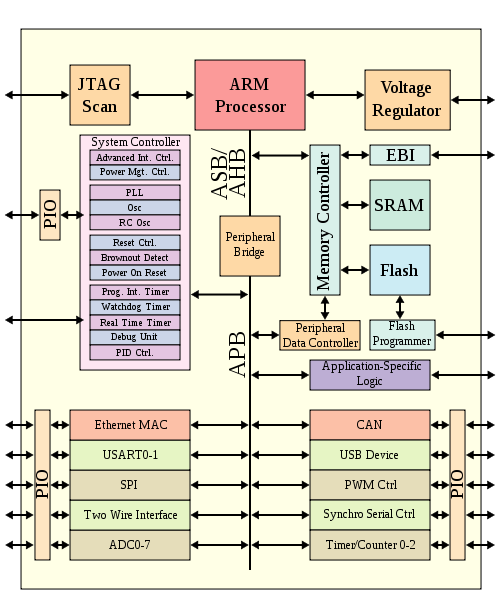
\includegraphics[width=0.5\textwidth]{Figures/ARM_SOC.png}
 % \caption[Diagrama de blocos de um soc ARM ]{Diagrama de blocos de um soc ARM }
 % \label{figures:ARM}
  %http://en.wikipedia.org/wiki/System_on_a_chip
%\end{figure}

%Os \acrshort{soc} têm uma vasta possibilidade de utilização desde um simples relógio até no mais avançado tecnologicamente como no desenvolvimentos de módulos para satélites, passando pela industria automóvel e com o aparecimento do arduino cada vez mais os \acrshort{soc} são utilizados em projetos de pequena escala desenvolvidos em casa, porque veio permitir a pessoas de com pouco ou nenhum conhecimento na área programar e efectuar debug no seu projecto com o \acrshort{soc}. A sua utilização traz vantagens com preço baixo, baixo consumo de energia e dimensões pequenas, como tudo o que existe também tem desvantagens sendo neste caso o baixo poder de calculo comparado com um computador. %http://www.extremetech.com/computing/126235-soc-vs-cpu-the-battle-for-the-future-of-computing

%Com uma área tão vasta de aplicações não é de estranhar que existam várias empresas \textcolor[rgb]{1,0,0}{a muito tempo} e varias startup no mercado a desenvolver \acrshort{soc} para fins totalmente distintos, cada empresa optimizando o seu para que foi desenvolvido.



% --------------------------------------------------------------------- 
\section{Modelo de Topo}
\label{section:Modelo de Topo}

O diagrama de topo do Versat é dado pela figura 3.1.

\begin{figure}[!htb]
  \centering
  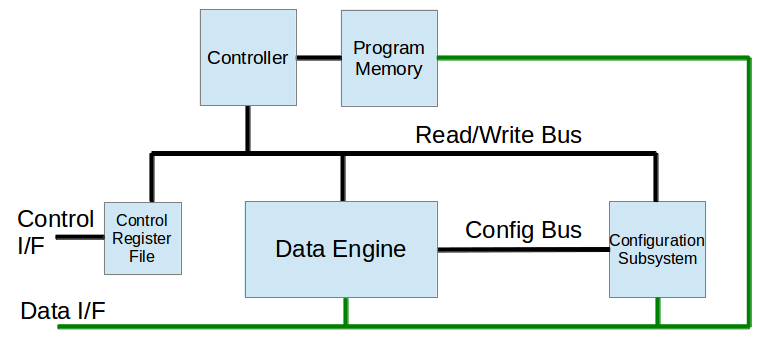
\includegraphics[height=80mm, width=165mm]{Figures/top.png}
  \caption[Esquema da unidade de topo.]{Esquema da unidade de topo.}  
  \label{fig:Esquema_Unidade_Topo}
\end{figure}

No Versat existem vários sub-componentes:

\begin{itemize}
  \item Data engine;
  \item Subsistema de configuração;
  \item Memória de instruções;
  \item Controlador;
  \item Ficheiro de registos de controlo;
  \item Descodificador de endereços;
  \item Sistema host-guest. 
\end{itemize}
%Uma startup no desenvolvimento de um projecto/produto necessita de um \acrshort{soc} para poder comercializar o seu produto. Na pesquisa do \acrshort{soc} ideal para o seu projecto encontram diferentes possibilidades, mas nenhuma preenchia todos os critérios pretendidos para o projecto. Como não foi encontrada uma solução ideal dos vários \acrshort{soc} disponíveis no mercado, a solução possível serias desenvolver o seu próprio \acrshort{soc} desenvolvido a medidas para o projecto.

O Versat é controlado centralmente pelo seu controlador. O controlador controla o barramento de Leitura/Escrita, que é usado para efectuar leitura/escrita nos registos dos outros sub-componentes. 


%\setlength{\parskip}{0 cm}



A interface de controlo é usada por um sistema {\it host}, que está a controlar o Versat. Os comandos são dados por um {\it host} e o Versat executa o que o {\it host} lhe ordena. Pela interface de controlo, são trocados preferencialmente comandos e informações de estado para indicar, por exemplo, o fim de algum comando executado. A troca de dados é realizada pela interface de dados. É também possível trocar dados pela interface de controlo, mas apenas quando a velocidade de transferência dos dados for pouco relevante. Por exemplo, caso o Versat esteja em modo de depuração, é usada a interface de controlo.

Existem dois tipos de barramentos de controlo possíveis de seleccionar: o barramento SPI e o barramento paralelo. 
O barramento SPI é usado quando se liga o Versat a um anfitrião externo, como por exemplo, um PC, para por exemplo, realizar a depuração de programas. O escravo SPI é o Versat, enquanto o mestre SPI é o anfitrião externo. 
O barramento paralelo é usado quando se liga o Versat a um anfitrião embebido. Este barramento está ligado ao ficheiro de registos de controlo e opera de uma forma simples e genérica. Pode ser necessário adaptar esta interface a um formato comercial, por exemplo, utilizando um barramento amba-AXI.


\section{Controlador}
\label{section:Controlador}

O controlador é descrito pela figura 3.2.

\begin{figure}[!htb]
  \centering
  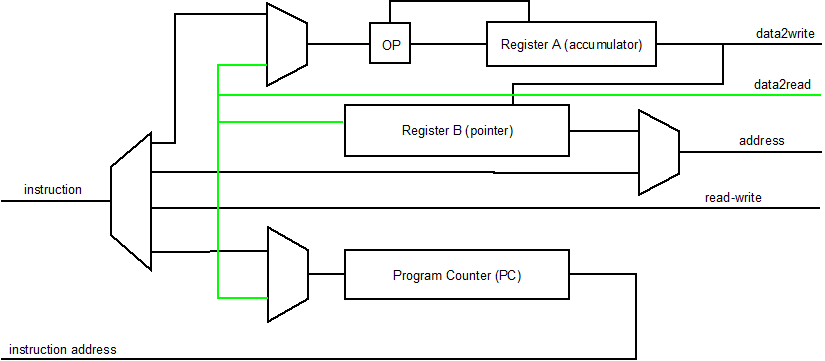
\includegraphics[height=110mm, width=155mm]{Figures/Controlador_MESMO.png}
  \caption[Esquema da unidade de controlo]{Esquema da unidade de controlo}  
  \label{fig:Esquema_Unidade_Controlo}
\end{figure}

\pagebreak

O controlador usa o barramento R/W para realizar leituras/escritas nos seus periféricos, que são módulos do Versat. A arquitectura do controlador do Versat é constituída por 3 registos:

\begin{itemize}
  \item Contador de programa;
  \item Acumulador (registo A);
  \item Apontador (registo B).
\end{itemize}

O contador de programa é usado como endereço da memória de instruções. A saída da memória de instruções contém a instrução que o controlador necessita de ler.

O Versat é uma arquitectura de acumulador. O registo A é o acumulador. O resultado de todas as operações realizadas pelo controlador vão parar ao acumulador, que armazena o valor.  
É no bloco OP que se efectuam as várias operações possíveis com o controlador. O bloco OP recebe como entrada o próprio acumulador e um dado de entrada de 32 {\it bits}. %onde se executa as instruções.  

O registo B é usado para endereçamento indirecto. O registo B guarda o endereço da próxima posição de memória a ler ou escrever numa instrução que utilize endereçamento indirecto. 


As funções principais do controlador são:

\begin{itemize}
  \item Comunicação com o sistema anfitrião;
  \item Implementação da estrutura de controlo dos procedimentos do Versat;
  \item Reconfiguração e controlo do Data Engine.
\end{itemize}

Caso o Versat esteja a trabalhar sozinho, em modo de depuração por exemplo, ele pode realizar o {\it upload}/{\it download} de dados e {\it upload} de procedimentos.

O controlador pode escrever na memória de instruções mas não pode ler da memória. Esta funcionalidade é usada para carregar procedimentos.
    
O controlador consegue ler e escrever no ficheiro de registos de controlo, que é partilhado com o sistema anfitrião. A função principal do ficheiro de registos de controlo é a de um canal de comunicação entre um anfitrião e o Versat. Os parâmetros necessários para correr os procedimentos no Versat são passados através deste canal.
    
O controlador pode escrever configurações parciais no subsistema de configuração de modo a reconfigurar o Data Engine. Também pode realizar pequenos cálculos que sejam necessários.

o conjunto de instruções executadas pelo controlador está descrito na tabela 3.1.

\pagebreak

\begin{table}[h!]
  \caption[Tabela das instruções assembly do Versat]{Tabela das instruções assembly do Versat}
  \begin{center}
    \begin{tabular}{|C{2cm}|c|c|c|}
      \hline
      {\bf Instruções} & {\bf Pseudo-código} \\
      \hline \hline
      nop & Nop \\
      \hline
      rdw & A $<$= (imm) \\
      \hline
      wrw & (imm) $<$= A \\
      \hline
      wrc & (imm1+imm2) $<$= A \\
      \hline
      rdwb & A $<$= (B) \\
      \hline 
      wrwb & (B) $<$= A \\
      \hline
      beqi & PC $<$= imm if regA=0\\
      \hline
      beq & PC $<$= (imm) if regA=0\\
      \hline
      bneqi & PC $<$= imm if regA!=0\\
      \hline
      bneq & PC $<$= (imm) if regA!=0\\
      \hline
      ldi & A $<$= imm \\
      \hline
      ldih & A[31:16] $<$= imm \\
      \hline
      add & A $<$= A + (imm) \\
      \hline
      addi & A $<$= A + imm\\
      \hline
      sub & A $<$= A - (imm)\\
      \hline 
      and & A $<$= A {\&} (imm) \\
     \hline
    \end{tabular}
  \end{center}
  \label{table:assembly_Versat}
\end{table}





%A startup no desenvolvimento de um projeto/produto necessita de um \acrshort{soc}, como se pode ver na figura \ref{grafos:problema} que tem de ter a capacidade de processamento necessária para efetuar a descodificação e codificação de dados que irá receber e enviar. O \acrshort{soc} desenvolvido tem de permitir que sejas ligado mais dois modelos assíncronos permitindo a recolha de dados no local para posterior envio dos dados pelo modelo de comunicação. O produto é para ser usado em locais de difíceis acessos este terá de ter um baixo consumo, permitindo que a bateria funcione o maior tempo possível. Para alem do mencionado anteriormente também necessita de duas interfaces de comunicação \acrlong{uart} e \acrlong{gpio}. 

%\begin{figure}[!htb]
 % \centering
 % 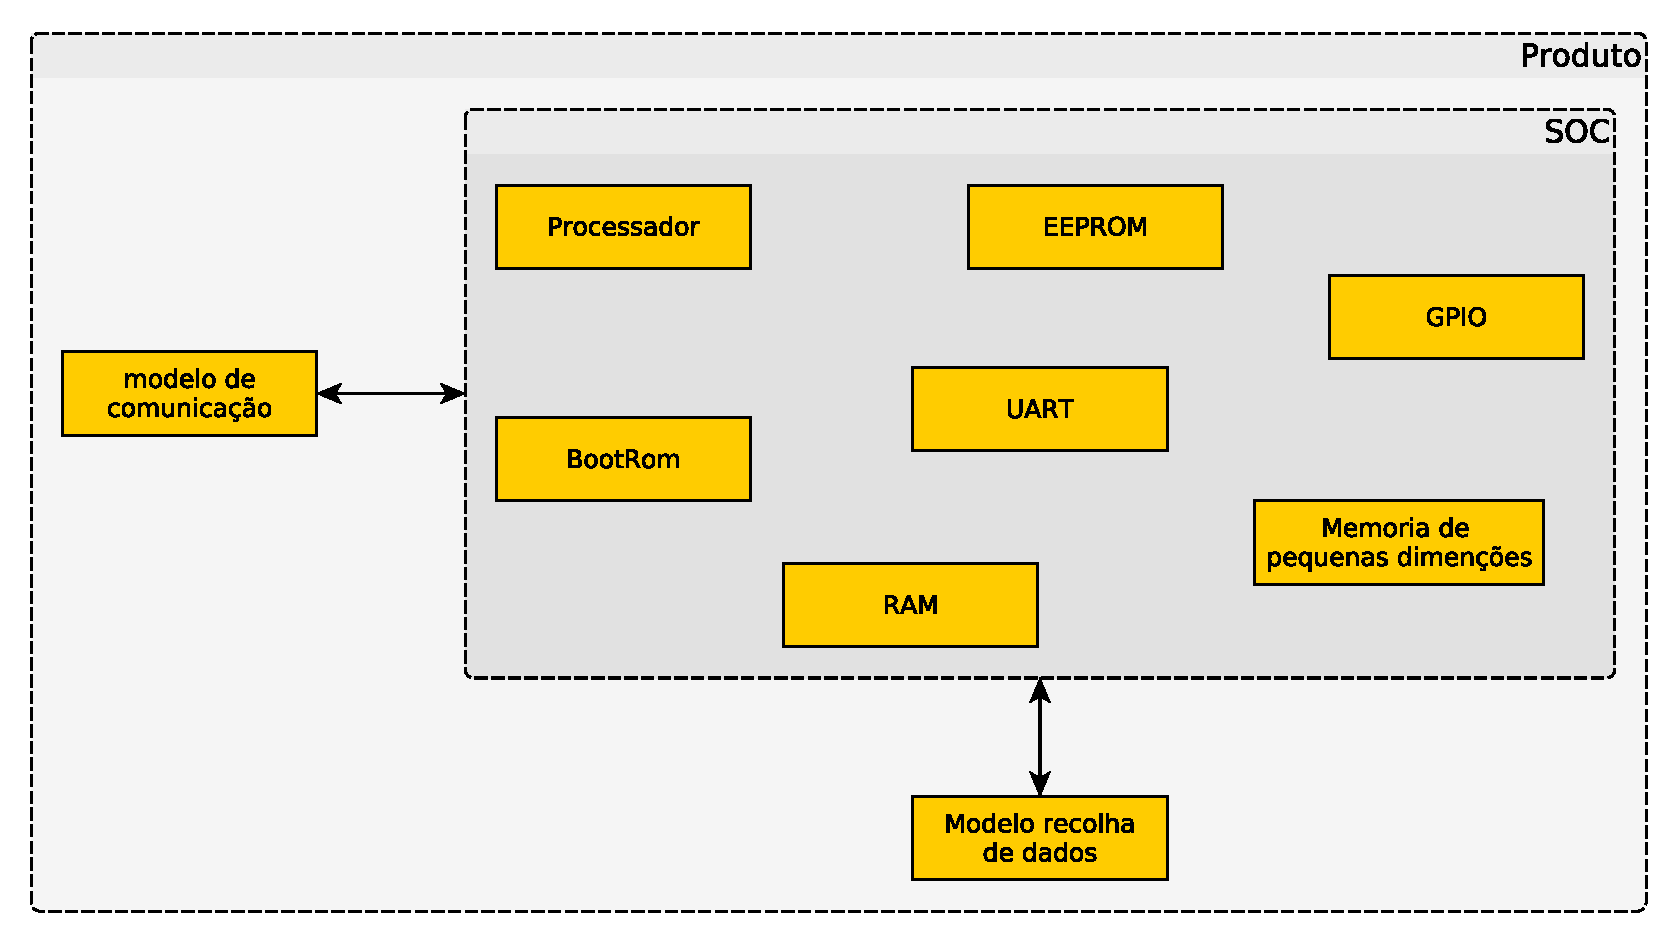
\includegraphics[width=0.5\textwidth]{grafos/problema.pdf}
 % \caption[SOC pretendido pela Startup]{SOC pretendido pela Startup}
 % \label{grafos:problema}
  %http://en.wikipedia.org/wiki/System_on_a_chip
%\end{figure}


\section{Data Engine}
\label{section:Data Engine}

O Data Engine é constituído por 15 unidades funcionais, organizadas como indicado na figura 3.3. A arquitectura usada tem 32 bits.



As memórias embebidas de porto duplo são memórias que têm um gerador de endereços por porto. É possível configurar cada um dos geradores de endereços de forma independente. Um gerador de endereços pode ser configurado com um número de iterações, período de cada iteração, incremento por ciclo, endereço de inicio e deslocamento entre períodos. 
As memórias podem ser configuradas para leitura ou escrita. No caso de serem configuradas para escrita, é necessário também configurar as entradas das memórias de modo a seleccionarem os dados certos.

As ALUs são unidades aritméticas lógicas que exercem diversas funções. As ALU-Lite executam apenas as primeiras 6 funções das ALUs, que são: 

\begin{itemize}
  \item OR lógico;
  \item AND lógico;
  \item NAND lógico;
  \item XOR lógico;
  \item Soma;
  \item Subtacção;
  \item Extensão de sinal de 8 para 32 bits;
  \item Extensão de sinal de 16 para 32 bits;
  \item SHIFT RIGHT aritmético;
  \item SHIFT RIGHT lógico;
  \item Comparação com sinal;
  \item Comparação sem sinal;
  \item Máximo; 
  \item Mínimo;
  \item Valor absoluto.
\end{itemize}

\begin{figure}[!htb]
  \centering
  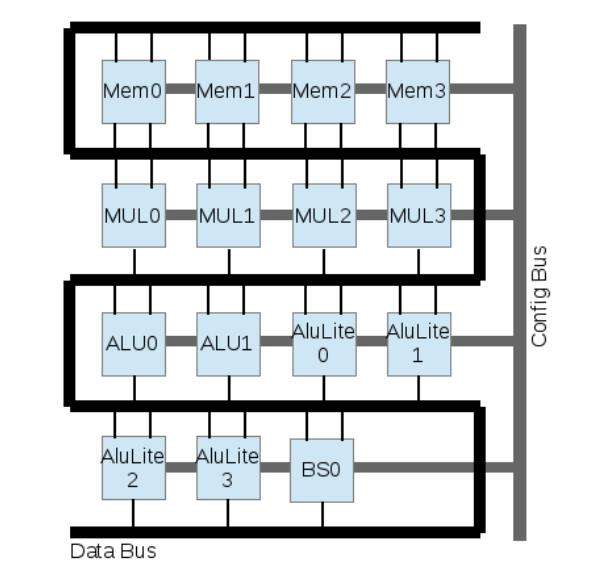
\includegraphics[height=130mm]{Figures/DataEngine.jpg}
  \caption[Esquema de ligações do Data Engine]{Esquema de ligações do Data Engine}  
  \label{fig:Esquema_ligacoes_DataEngine}
\end{figure}

Os multiplicadores efectuam uma multiplicação de dois operandos de 32 bits com um resultado de 64 bits, do qual só 32 bits são utilizados. É possível escolher se se quer a parte alta da multiplicação (bit 32 ao bit 63) ou a parte baixa (bit 0 ao bit 31). Também é possível escolher efectuar ou não a divisão por 2 do resultado final, o que ajuda quando se trabalha em notações de vírgula fixa.

Os {\it shifters} são unidades especializadas em deslocamento de bits. Um dos operandos é a palavra a deslocar e o outro operando é a magnitude do deslocamento. Os {\it shifters} são configurados com o sentido de deslocamento (esquerda ou direita) e o tipo de deslocamento (aritmético ou lógico).

Cada unidade de processamento contribui com 32 bits para o Data Bus. Cada unidade de processamento é capaz de seleccionar qualquer secção de 32 bits existente no Data Bus, o que permite que todas as unidades de processamento possam estar interligadas umas às outras. Isto facilita o trabalho do compilador, que não precisa de fazer {\it Place and Route}. 

As unidades de processamento são configuradas com o modo de operação e com as respectivas entradas. Não existem configurações globais, todas as configurações existentes são acerca de cada FU independente. Cada conjunto de unidades de processamento configuradas origina um datapath para uma tarefa específica.


Se num {\it datapath} estiverem várias memórias, as memórias vão trabalhar em sincronismo. Se existirem recursos suficientes, mais do que um {\it datapath} pode executar em paralelo, permitindo realizar paralelismo ao nível de tarefa. 

Para controlar o Data Engine, é necessário atribuir valores no seu registo de controlo, tal como descrito na tabela~\ref{tab:de_ctr_reg}. Pode essencialmente inicializar-se as unidades de processamento (bit 0, Init) ou manda-las correr (bit 1, Run). 
Os restantes bits deste registo (bit 2 a 20) indicam quais as unidades de processamento a inicializar ou correr. A inicialização de memórias tem como resultado o carregamento das configurações dos registos de endereços. A inicialização de outras unidades funcionais têm como resultado o anulamento do valor de saída.
Mandar correr as memórias faz iniciar a geração de endereços nas memórias indicadas. Mandar correr qualquer outra unidade de processamento tem apenas o efeito de anular as suas saídas inicialmente. 

\begin{table}[!htbp]
   \caption{Registo de controlo do Data Engine.}
  \centering
    \begin{tabular}{|p{1.5cm}|p{7cm}|}
    \hline 
    {\bf Bit} & {\bf Descrição} \\
    \hline \hline 
     0 & Init \\
    \hline
     1 & Run \\
    \hline
     2 & BS0 \\
    \hline
     3 & Mult3 \\
    \hline
     4 &  Mult2\\
    \hline
     5 &  Mult1  \\
    \hline
     6 & Mult0 \\
    \hline
     7 & ALULite3 \\
    \hline
     8 & ALULite2 \\
    \hline
     9 &  ALULite1\\
    \hline
     10 & ALULite0 \\
    \hline
     11 & ALU1 \\
    \hline
     12 & ALU0\\
    \hline
     13 & MEM3B \\
    \hline
     14 & MEM3A \\
    \hline
     15 &  MEM2B\\
    \hline
     16 &  MEM2A\\
    \hline
     17 &  MEM1B\\
    \hline
     18 &  MEM1A\\
    \hline
     19 &  MEM0B\\
    \hline
     20 &  MEM0A\\
    \hline
     21-31 & Reserved \\
    \hline
    \end{tabular}
  \label{tab:de_ctr_reg}
\end{table}

Quando se manda correr o Data Engine é necessário saber quando a sua operação termina. Para tal usa-se o registo de estado do Versat descrito na tabela~\ref{tab:de_stat_reg}. Este registo indica quais as memórias que terminaram a sua sequência de endereços.


\begin{table}[!htbp]
  \centering
  \caption{DE status register.}
    \begin{tabular}{|p{1.5cm}|p{7cm}|}
    \hline 
    {\bf Bit} & {\bf Description} \\
    \hline \hline 
     0 & MEM0B done \\
    \hline
     1 & MEM0A done\\
    \hline
     2 & MEM1B done \\
    \hline
     3 & MEM1A done \\
    \hline
     4 & MEM2B done \\
    \hline
     5 & MEM2A done  \\
    \hline
     6 & MEM3B done \\
    \hline
     7 & MEM3A done \\
    \hline
     8-31 & Reserved \\
    \hline

    \end{tabular}
  \label{tab:de_stat_reg}
\end{table}


\section{Subsistema de configuração}
\label{section:Subsistema de configuracao}

O subsistema de configuração é um sistema de memória onde as configurações do Data Engine estão guardadas. 

A configuração principal está guardada num registo parcialmente endereçado. Existe também uma réplica do registo de configuração principal (registo sombra) que permite manter a configuração do Data Engine enquanto que o registo de configuração principal é modificado para conter a próxima configuração. 
Existe também uma memória de configurações que permite armazenar configurações utilizadas frequentemente. Deste modo, após a escrita de uma configuração para o registo principal, e após a sua utilização no Data Engine, pode-se guardar o seu valor na memória de configurações para reutilização mais tarde.




\section{Memória de instruções}
\label{section:Memoria de instrucoes}

A memória de instruções é constituída por uma memória RAM e uma memória ROM. A memória RAM tem 2048 posições enquanto que a ROM tem 256 posições. No futuro poderá ser necessário aumentar o tamanho da memória, ou transforma-la numa cache, pois o uso de compiladores pode produzir código pouco optimizado.

O carregamento das instruções realiza-se numa fase de {\it setup}, antes de se usar o Versat. O carregamento das instruções é feita através da interface de dados entre o controlador do Versat e o exterior. 

A ROM (também designada de boot ROM) contém um programa fixo para carregamento de programas do Versat, dados e para executar programas previamente carregados. A boot ROM também pode ser usada para descarregar dados calculados pelo Versat. A RAM é usada após o carregamento do programa, para executar esse mesmo programa. 


\cleardoublepage






%Os principais desafios desta dissertação consiste no desenvolvimento de um sistema sintetizável que preencha todas as necessidades mencionadas pela startup.

%Desenvolver uma interface assíncrona necessária para a comunicação entre o \acrshort{soc} e os modelos de comunicação e de recolha de dados a ser desenvolvido pela startup.

%A criação de uma bootrom que carregua para a memoria principal o programa que se encontra na EEPROM. Ainda testa o mau funcionamento da EEPROM ou da memoria principal notificando o utilizador. 
 % Thesis_Spi.tex

%%%%%%%%%%%%%%%%%%%%%%%%%%%%%%%%%%%%%%%%%%%%%%%%%%%%%%%%%%%%%%%%%%%%%%%%
%                                                                      %
%     File: Thesis_Introduction.tex                                    %
%     Tex Master: Thesis.tex                                           %
%                                                                      %
%     Author: Rui Santiago                         			   %
%     Last modified : 2 Junho 2015                         		   %
%                                                                      %
%%%%%%%%%%%%%%%%%%%%%%%%%%%%%%%%%%%%%%%%%%%%%%%%%%%%%%%%%%%%%%%%%%%%%%%%

\chapter{Compilador básico}
\label{chapter:Compilador basico}

Existem duas abordagens possíveis para realizar o compilador: fazer uma compilação clássica, através da construção de árvores de sintaxe abstracta ({\it abstract syntax trees}), cada uma representando uma expressão, realizando a respectiva decomposição e gerando as várias instruções. 

Outra abordagem que é analisada neste capítulo é fugir à implementação de um compilador clássico e utilizar uma linguagem de orientação por objectos para representar os componentes de {\it hardware}, onde cada classe é um componente de {\it hardware}. 
O programador utiliza essas classes com o objectivo de configurar o Data Engine.

Os métodos das classes permitem que o programador utilize as várias funções dos componentes de {\it hardware}. O programador utiliza as classes para descrever acções de controlo ou estruturas de {\it hardware} que permitam realizar a tarefa em questão.

O objectivo é construir uma linguagem de muito baixo nível para depois com o passar do tempo ser possível subir o nível de abstracção. 


\section{Abordagem da construção das árvores de sintaxe abstracta}
\label{section:Abordagem da construcao das arvores de sintaxe abstracta}

Construindo árvores de sintaxe abstracta é possível descodificar as expressões em instruções e gerar o respectivo {\it assembly}. A árvore de sintaxe abstracta é usada para analisar gramaticalmente as expressões. 

\subsection{Soma simples}
\label{subsection:Soma simples}

Considerando a soma de dois registos:

\begin{lstlisting} 
       R5 = R1+R2;      
\end{lstlisting}  
    
A árvore de análise respectiva encontra-se na figura~\ref{fig:Arvore_de sintaxe abstracta_de_uma_soma}.
No momento da construção da árvore, a árvore é percorrida da esquerda para a direita. A descodificação é feita pela seguinte ordem:

\begin{itemize}
  \item Entrada em R1 e memorização da instrução RDW, que vai executar uma leitura;
  \item Entrada em +, memorizando a instrução ADD;
  \item Entrada em R2, que vai indicar qual o regsto que se vai somar ao conteúdo do registo A;
  \item Gravar o resultado em R5, memorizando a instrução WRW.
\end{itemize}
    
    \begin{figure}[!htb]
  \centering
  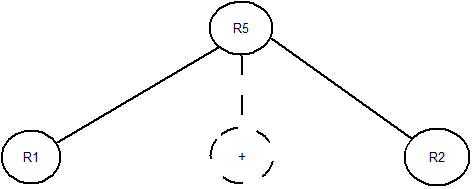
\includegraphics[height=45mm]{Figures/grafo1.png}
  \caption[Árvore lexical de uma soma.]{Árvore de sintaxe abstracta de uma soma.}  
  \label{fig:Arvore_de sintaxe abstracta_de_uma_soma}
\end{figure}
    
    O resultado é apenas gravado quando se termina a recursividade.
O respectivo código {\it assembly} é:

    RDW R1    

    ADD R2

    WRW R5
    
Esta abordagem é boa para compilar expressões para o controlador controlador, pois o controlador funciona como uma máquina convencional. No entanto, 
é uma abordagem menos boa para configurar e controlar o Data Engine.

\subsection{Ciclo {\it for}}
\label{subsection:Ciclo for}

Para a realização de um ciclo {\it for}, é necessário o uso do Data Engine. Considera-se o caso do ciclo {\it for} seguinte:

\begin{lstlisting}
    for (i=0;i<N;i++)    {
       MEM3[i] = MEM2[2i]+MEM2[2i+1];      }
\end{lstlisting}

Para o uso de ciclos {\it for}, não é necessário fazer a decomposição das expressões em instruções {\it assembly} usando compilação clássica, pois o Data Engine funciona de maneira diferente do controlador. No Data Engine usa-se instruções {\it assembly} apenas para sua configuração,
enquanto que no controlador cada expressão é descodificada para um equivalente em {\it assembly} para a execução. 
Conclui-se assim que para o Data Engine as árvores de sintaxe abstractas não são muito úteis.

\clearpage

\begin{figure}[!htb]
  \centering
  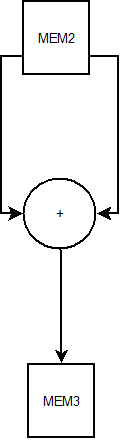
\includegraphics[height=90mm]{Figures/grafo2.png}
  \caption[Árvore lexical de uma soma]{Árvore lexical de uma soma dentro de um ciclo for}  
  \label{fig:Arvore_lexical_de_uma_soma_no_ciclo_for}
\end{figure}

Para o uso do Data Engine, é necessário usar um grafo em vez de uma árvore de sintaxe abstracta. Para um exemplo dado acima, construiu-se o grafo mostrado na figura~\ref{fig:Arvore_lexical_de_uma_soma_no_ciclo_for}. O compilador teria de identificar este grafo e depois controlar a execução do Data Engine. 

O código {\it assembly} que deveria ser produzido é dado a seguir:

\begin{lstlisting}
#clear conf_reg
	wrw CLEAR_CONFIG_ADDR
#configure mem2 for reading vectors x1 and x2
	ldi 0
	wrc MEM2A_CONFIG_ADDR,MEM_CONF_START_OFFSET
	ldi 1
	wrc MEM2B_CONFIG_ADDR,MEM_CONF_START_OFFSET
	ldi 1
	wrc MEM2A_CONFIG_ADDR,MEM_CONF_DUTY_OFFSET
	wrc MEM2B_CONFIG_ADDR,MEM_CONF_DUTY_OFFSET
	wrc MEM2A_CONFIG_ADDR,MEM_CONF_PER_OFFSET
	wrc MEM2B_CONFIG_ADDR,MEM_CONF_PER_OFFSET
	ldi 2
	wrc MEM2A_CONFIG_ADDR,MEM_CONF_INCR_OFFSET
	wrc MEM2B_CONFIG_ADDR,MEM_CONF_INCR_OFFSET
	ldi N
	wrc MEM2A_CONFIG_ADDR,MEM_CONF_ITER_OFFSET
	wrc MEM2B_CONFIG_ADDR,MEM_CONF_ITER_OFFSET
#configure mem3 for writing result
	ldi salu0
	wrc MEM3A_CONFIG_ADDR,MEM_CONF_SELA_OFFSET
	ldi 0
	wrc MEM3A_CONFIG_ADDR,MEM_CONF_START_OFFSET
	ldi 1
	wrc MEM3A_CONFIG_ADDR,MEM_CONF_DUTY_OFFSET
	wrc MEM3A_CONFIG_ADDR,MEM_CONF_PER_OFFSET
	wrc MEM3A_CONFIG_ADDR,MEM_CONF_INCR_OFFSET
	ldi 6
	wrc MEM3A_CONFIG_ADDR,MEM_CONF_DELAY_OFFSET
	ldi N
	wrc MEM3A_CONFIG_ADDR,MEM_CONF_ITER_OFFSET
#configure alu0 for adding x1 and x2
	ldi ALU_ADD
	wrc ALU0_CONFIG_ADDR,ALU_CONF_FNS_OFFSET
	ldi smul1
	wrc ALU0_CONFIG_ADDR,ALU_CONF_SELA_OFFSET
	ldi salu0
	wrc ALU0_CONFIG_ADDR,ALU_CONF_SELB_OFFSET
	ldi 1
#init engine
	ldi 0xfffd
	ldih 1
	wrw ENG_CTRL_REG
	wrw ENG_CTRL_REG
#run engine
	ldi 0xc002 
	ldih 1 
	wrw ENG_CTRL_REG
#wait for completion to display results
waitres	ldi 256
	and ENG_STATUS_REG
	beqi waitres
	nop
	nop
#branch to boot ROM
	ldi 0
	beqi 0
	nop
	nop
\end{lstlisting}

O número de iterações é definido por N, que é necessário indicar nos parâmetros \linebreak MEM{\_}CONF{\_}ITER{\_}OFFSET de cada memória usada. Visto que o i inicial é zero por pré-definição no compilador desenvolvido, 
os parâmetros MEM{\_}CONF{\_}INCR{\_}OFFSET e MEM{\_}CONF{\_}START{\_}OFFSET são usados para calcular os endereços na memória X da seguinte forma:

MEMx[INCR{\_}OFFSET*i+START{\_}OFFSET]

O gerador de endereços usado entre os dois disponíveis em cada memória é indicado pelo programador. Numa primeira abordagem, o período de cada iteração será também definido pelo programador. No futuro poderão usar-se mecanismos para automatizar o cálculo do período.

Os valores usados para inicializar e correr o Data Engine serão calculados internamente pelo compilador, recebendo instruções mais simples do utilizador. 

No ciclo {\it waitres} é usada uma máscara consoante a memória que se quer monitorizar. Quando uma memória acaba de ser lida ou escrita, é indicado no ENG{\_}STATUS{\_}REG que a memória terminou a sua execução.



\section{Utilização de uma linguagem orientada a objectos}
\label{section:Utilizacao de uma linguagem orientada a objectos}


A outra abordagem é através do uso de várias classes que representem os componentes do {\it Data Engine}. Utilizando esta abordagem, o programador escreve um programa com as classes disponíveis, descrevendo várias configurações do Data Engine.
Para as instruções do controlador, é usada uma linguagem interpretada. O UML das classes usadas no Data Engine é dado na figura~\ref{fig:tese_UML}.

%\begin{figure}[!htb]
 % \centering
 % 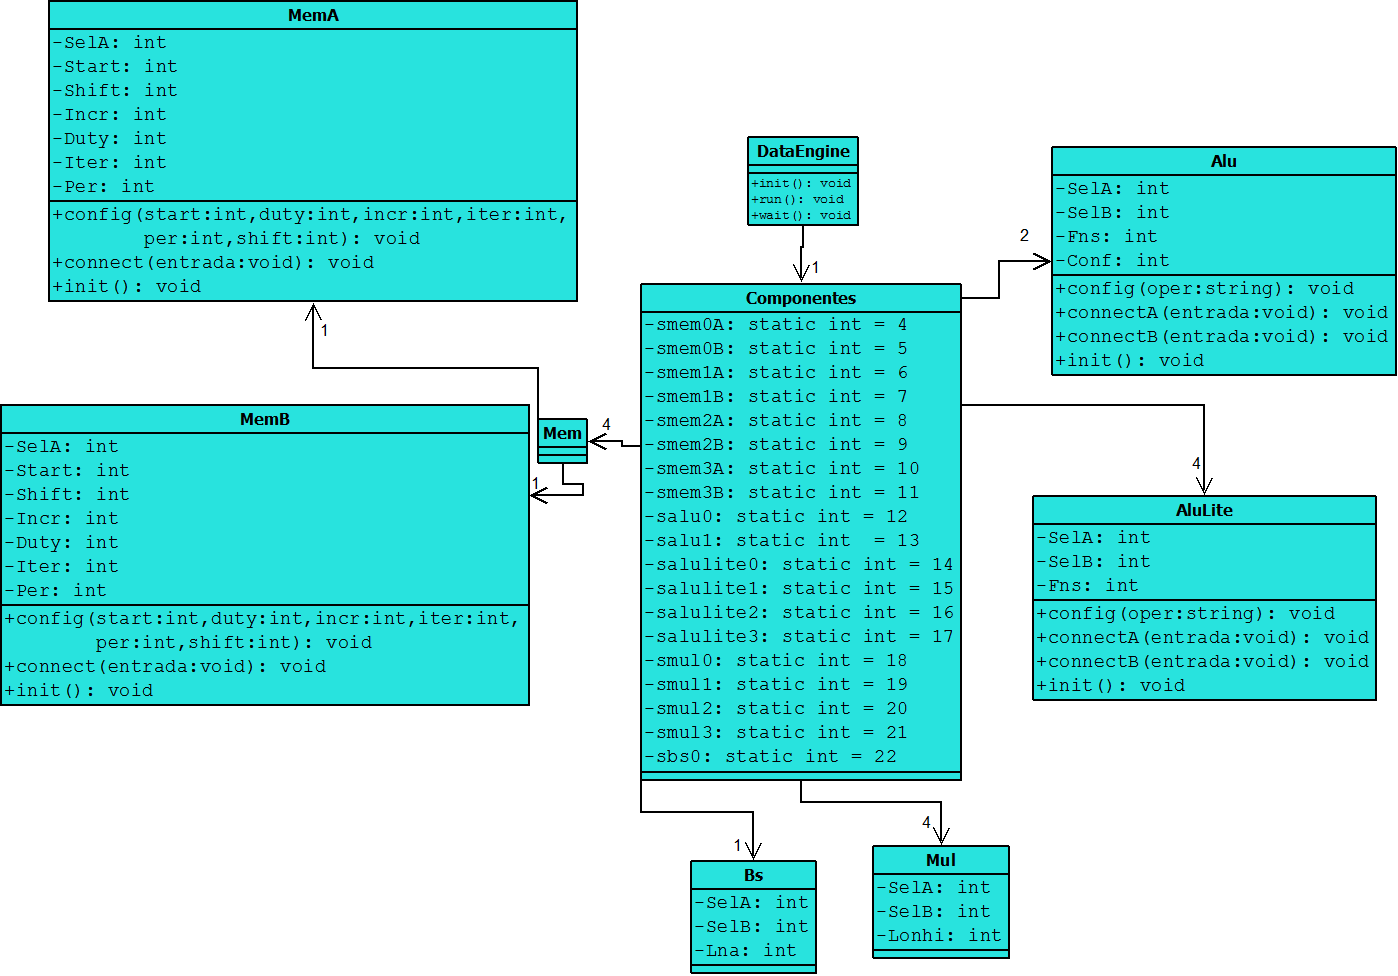
\includegraphics[height=175mm, angle=270, width=155mm]{Figures/tese_UML.png}
 % \caption[UML do Data Engine.]{UML do Data Engine.}  
%  \label{fig:tese_UML}
%\end{figure}

A compilação do código será feita pelo script automaticamente. Cada classe construirá o seu respectivo {\it Assembly}.

A nível do {\it Data Engine}, as ligações serão feitas directamente nas classes, que usando métodos do {\it Data Engine}, geram o próprio {\it Assembly}. 


%Para correr a instrução \begin{lstlisting} 
  %     R5 = R1+R2;      
%\end{lstlisting} é apenas necessário fazer

%R5=R1+R2





Considerando o exemplo da soma vectorial da secção anterior, o respectivo pseudo-código na linguagem Versat é:

\begin{lstlisting}

mem2A.config(0, 1, 2, N, 1, 0); // inicializar a memoria 2A
mem2B.config(1, 1, 2, N, 1, 0); // inicializar a memoria 2B
mem3A.config(0, 1, 6, N, 1, 0); // inicializar a memoria 3A

alu0.config("ADD"); // inicializar a alu

alu0.connectA(mem2A); // conectar a entrada A da alu a mem2A
alu0.connectB(mem2B); // conectar a entrada B da alu a mem2B

mem3A.connect(alu0); // conectar a memoria 3A a saida da ALU

mem2A.init(); // inicializar a memoria 2A
mem2B.init(); // inicializar a memoria 2B
mem3A.init(); // inicializar a memoria 3A
alu0.init(); // inicializar a alu0

mem3A.wait(); // marcar esta memoria para que se espere por ela


engine.init();
engine.run();
engine.wait();


\end{lstlisting}

Nos métodos de configuração das memórias, é passado o início, o
período, o {\it duty}, o incremento, o {\it delay} e o número de
iterações. De início decidiu-se passar também o {\it delay} mas
poderão vir a ser experimentadas formas de o compilador calcular o
{\it delay}.  A ALU precisa apenas de saber qual a operação que vai
realizar.

As conexões são feitas utilizando métodos do objecto destino. Existe
um método para cada conexão, um para a entrada A e outro para a
entrada B.

Como se pode ver, a descrição acima, usando um paradigma de
programação por objectos, consegue realizar a mesma função que o
código {\it assembly} dado para este exemplo. A diferença é que se
consegue uma descrição muito mais compacta e fácil de ler quando se
usa uma representação por objectos.

Poderia pensar-se em usar qualquer linguagem de programação orientada
para objectos para realizar descrições de configurações do Data Engine
e do seu controlo. Até se poderia usar uma linguagem de {\it
  scripting} como Python, a qual tem suporte para classes e
métodos. Estes programas quando executados gerariam o código assembly
ou o código máquina directamente. Esta abordagem evitaria de todo o
desenvolvimento de um {\em parser} para o compilador do Versat.

Contudo, uma parte importante do problema é compilar o código que é
corrido pelo controlador do Versat. Uma linguagem para esse fim seria
próxima de uma linguagem de programação convencional e teria de
incluir expressões condicionais ({\it if}) e ciclos de programa ({\it
  for, while, do while}, etc). Estas expressões são mais difíceis de
traduzir apenas chamando métodos de classes, e mesmo que se arranjasse
uma solução para tal, o código produzido não seria compacto e
elegante.


\begin{figure}[!htb]
  \centering
  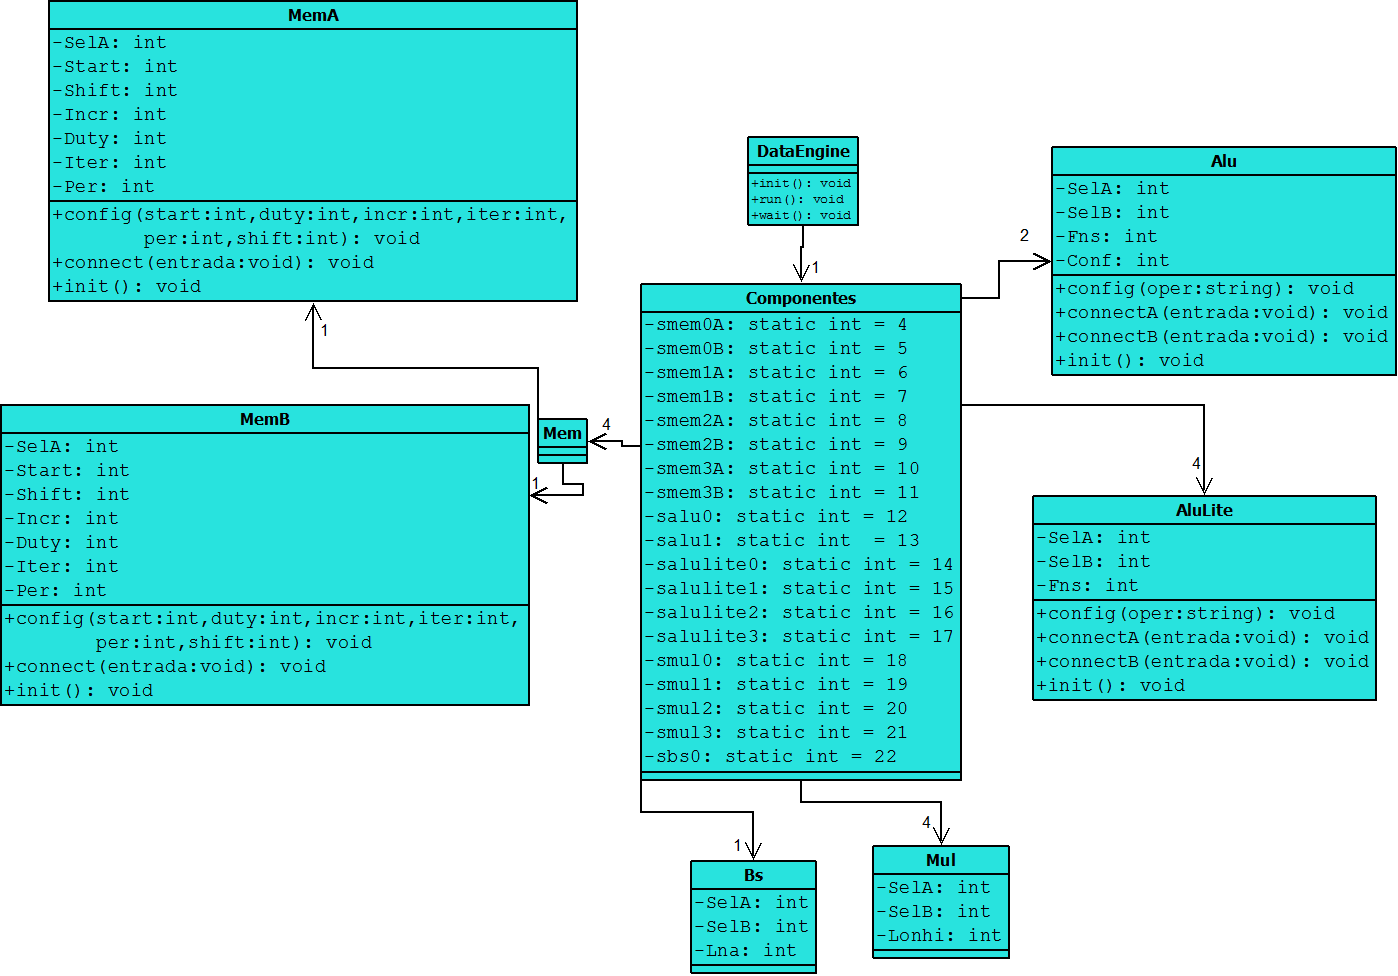
\includegraphics[height=105mm, angle=270, width=155mm]{Figures/tese_UML.png}
  \caption[UML do Data Engine.]{UML do Data Engine.}  
  \label{fig:tese_UML}
\end{figure}

\cleardoublepage
 % Thesis_I2C.tex

%%%%%%%%%%%%%%%%%%%%%%%%%%%%%%%%%%%%%%%%%%%%%%%%%%%%%%%%%%%%%%%%%%%%%%%%
%                                                                      %
%     File: Thesis_Introduction.tex                                    %
%     Tex Master: Thesis.tex                                           %
%                                                                      %
%     Author: Rui Santiago                         			   %
%     Last modified : 4 Junho 2015                      		   %
%                                                                      %
%%%%%%%%%%%%%%%%%%%%%%%%%%%%%%%%%%%%%%%%%%%%%%%%%%%%%%%%%%%%%%%%%%%%%%%%


\chapter{Resultados}
\label{chapter:Resultados}





\cleardoublepage
 % Thesis_I2C.tex

%%%%%%%%%%%%%%%%%%%%%%%%%%%%%%%%%%%%%%%%%%%%%%%%%%%%%%%%%%%%%%%%%%%%%%%%
%                                                                      %
%     File: Thesis_Conclusions.tex                                     %
%     Tex Master: Thesis.tex                                           %
%                                                                      %
%     Author: Carlos A. Rodrigues                                      %
%     Last modified : 21 Jan 2011                                      %
%                                                                      %
%%%%%%%%%%%%%%%%%%%%%%%%%%%%%%%%%%%%%%%%%%%%%%%%%%%%%%%%%%%%%%%%%%%%%%%%

\chapter{Conclusão}
\label{chapter:conclusao}

Insert your chapter material here...


% ----------------------------------------------------------------------
\section{Achievements}
\label{section:achievements}

The major achievements of the present work...


% ----------------------------------------------------------------------
\section{Trabalho Futuro}
\label{section:futuro}

dese


\cleardoublepage

 % file "Thesis_Conclusions.tex"

% ----------------------------------------------------------------------
%  Appendix (optional)
% ----------------------------------------------------------------------
%\appendix
%%%%%%%%%%%%%%%%%%%%%%%%%%%%%%%%%%%%%%%%%%%%%%%%%%%%%%%%%%%%%%%%%%%%%%%%%
%                                                                      %
%     File: Thesis_Appendix.tex                                        %
%     Tex Master: Thesis.tex                                           %
%                                                                      %
%     Author: Carlos A. Rodrigues                                           %
%     Last modified : 21 Jan 2011                                      %
%                                                                      %
%%%%%%%%%%%%%%%%%%%%%%%%%%%%%%%%%%%%%%%%%%%%%%%%%%%%%%%%%%%%%%%%%%%%%%%%

\chapter{Vector calculus}
\label{chapter:appendixVectors}

In case an appendix if deemed necessary, the document cannot exceed a total of 100 pages...

Some definitions and vector identities are listed in the section below.

% ----------------------------------------------------------------------
\section{Vector identities}
\label{section:vectorIdentities}

\begin{equation}
	\nabla \times \left( \nabla \phi \right) = 0
	\label{eq:cross_nnp}
\end{equation}

\begin{equation}
	\nabla \cdot \left( \nabla \times {\bf u} \right) = 0
	\label{eq:dotCross_nnu}
\end{equation}

\cleardoublepage

 % file "Thesis_Appendix.tex"

% ----------------------------------------------------------------------
%  Bibliography
% ----------------------------------------------------------------------

% Include all references in .bib file, even non-cited ones...
%\nocite{*}

% Produces the bibliography section when processed by BibTeX
%
% Bibliography style
% > entries ordered alphabetically
%\bibliographystyle{plain}
% > unsorted with entries appearing in the order in which the citations appear.
\bibliographystyle{unsrt}
% > entries ordered alphabetically, with first names and names of journals and months abbreviated
%\bibliographystyle{abbrv}
% > entries ordered alphabetically, with reference markers based on authors' initials and publication year
%\bibliographystyle{alpha}
%
% Replacement bibliography styles provided by 'natbib' package
% (plainnat.bst, abbrvnat.bst, unsrtnat.bst )
% > entries ordered alphabetically
%\bibliographystyle{plainnat}
% > unsorted with entries appearing in the order in which the citations appear.
%\bibliographystyle{unsrtnat}
% > entries ordered alphabetically, with first names and names of journals and months abbreviated
%\bibliographystyle{abbrvnat}
% > entries ordered alphabetically, with reference markers based on authors' initials and publication year
%\bibliographystyle{alpha}


% External bibliography database file in the BibTeX format
\cleardoublepage
\bibliography{Thesis_bib_DB} % file "Thesis_bib_DB.bib"
% Add entry in the table of contents as chapter
\addcontentsline{toc}{chapter}{\bibname}
\cleardoublepage

% ----------------------------------------------------------------------
\end{document}
% ----------------------------------------------------------------------

